\documentclass[12pt]{article}

\setlength{\topmargin}{-.75in} \addtolength{\textheight}{2.00in}
\setlength{\oddsidemargin}{.00in} \addtolength{\textwidth}{.75in}

\usepackage{amsmath,color,graphicx,array,multirow,rotating, enumerate}
\usepackage{type1cm}
\usepackage{eso-pic}
\usepackage[hmargin=2cm,vmargin=1.3cm]{geometry}
\usepackage{mathabx}
\usepackage[rflt]{/Users/jgates/desktop/latex/floatflt}
\usepackage[table]{xcolor}
\nofiles

\def\Tab#1{\tabular[t]{>{\rule[-1ex]{0pt}{3ex}}c}#1\endtabular}
\newcolumntype{C}{@{}c@{}}

\pagestyle{empty}
\newcounter{ProbNum}
\setlength{\parindent}{0in}

% Watermark: graph paper
\newcommand\BackgroundPic{
\put(0,0){
\parbox[b][\paperheight]{\paperwidth}{%
\vfill
\centering

\includegraphics[width=\paperwidth,height=\paperheight,keepaspectratio]{/Users/jgates/desktop/latex/pics/plain.pdf}%
\vfill
}}}

%Diagram box command [v space][content]
\newcommand{\diagrambox}[2][40 mm]{
\framebox{\parbox{175 mm}{#2 \hfill \\ \vspace{#1}}}

\bigskip
}

% MakeList: [example number] [content]
\newcommand{\MakeList}[2]{
\begin{enumerate}[#1] \itemsep1pt \parskip0pt \parsep0pt  

#2
\end{enumerate}
}

\begin{document}



{\Large All problems:}
\bigskip 
% Number 1
% BFPM Tension FBD Vectors
% Hanging box, rope around 2 pulleys, theta = phi

% Watermark
\AddToShipoutPicture*{\BackgroundPic}

\addtocounter {ProbNum} {1}

\begin{floatingfigure}[r]{.2\textwidth}
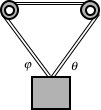
\includegraphics[scale=1]{/Users/jgates/desktop/latex/pics/hangingbox1.png}
\end{floatingfigure}
 
{\bf \Large{1.}} The box of mass ${6~kg}$ hangs at rest. 

\bigskip

\indent  a. Prove that ${\theta = \varphi}$.

\bigskip 
b. Determine the tension in the rope, if ${\theta = 50^\circ}$.

\bigskip 
\vspace{6mm}% Number 10
% Vectors
% Trig review - box leaning on wall
% MIT Physics for Teachers LON-CAPA

% Watermark
\AddToShipoutPicture*{\BackgroundPic}

\addtocounter {ProbNum} {1}

\begin{floatingfigure}[r]{.3\textwidth}
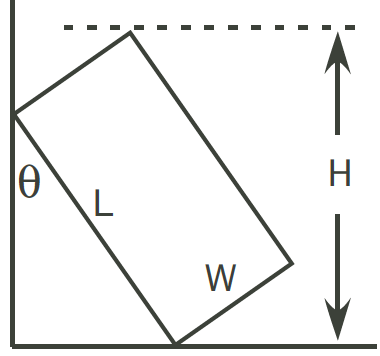
\includegraphics[scale=.4]{/Users/jgates/desktop/latex/pics/leaningbox.png}
\end{floatingfigure}
 
{\bf \Large{10.}} A rectangular box of length $L$ and width $W$ rests against a wall, making an angle $\theta$ with respect to the wall.  

\bigskip

\indent What is the height $H$ of the top edge of the box above the floor?

\bigskip 
\vspace{6mm}% Number 100
% CAPM AMM
% Car speeds up, slows down: rel. easy, pairs with 90
% MIT Physics for Teachers LON-CAPA

% Watermark
\AddToShipoutPicture*{\BackgroundPic}

\addtocounter {ProbNum} {1}

%\begin{floatingfigure}[r]{.3\textwidth}
%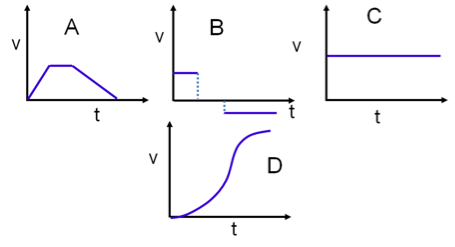
\includegraphics[scale=.4]{/Users/jgates/desktop/latex/pics/vgraph1.png}
%\end{floatingfigure}
 
{\bf \Large{100.}} A car starting from rest speeds up to ${30~\frac{m}{s}}$ with constant acceleration in 15 seconds. Then, it travels at ${30~\frac{m}{s}}$ for 10 seconds. Finally, it brakes to a stop in 30 seconds with constant acceleration. 

 \bigskip

\indent How far does it travel in the 55 second time period?  
 

\bigskip 
\vspace{6mm}% Number 110
% CAPM Motionmap
% Car speeds up, slows down: MC pick motion map
% MIT Physics for Teachers LON-CAPA

% Watermark
\AddToShipoutPicture*{\BackgroundPic}

\addtocounter {ProbNum} {1}

\begin{floatingfigure}[r]{.3\textwidth}
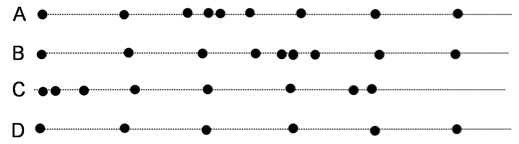
\includegraphics[scale=.4]{/Users/jgates/desktop/latex/pics/Motionmap1.png}
\end{floatingfigure}
 
{\bf \Large{110.}} Driving a car in the positive x direction at a speed of 60 mph, Mary tests her brakes by coming to a complete stop in 4 seconds. Then she accelerates to her original speed of 60 mph in 8 seconds. A motion diagram is created by illuminating her car with a strobe at 2 second intervals. 

 \bigskip

\indent Which of the following best represents the correct diagram? Mary�s car is represented by a dot.   
 

\bigskip 
\vspace{6mm}% Number 120
% BFPM Vectors Friction
% Force diagram MC on incline, bad lengths
% MIT Physics for Teachers LON-CAPA

% Watermark
\AddToShipoutPicture*{\BackgroundPic}

\addtocounter {ProbNum} {1}

\begin{floatingfigure}[r]{.3\textwidth}
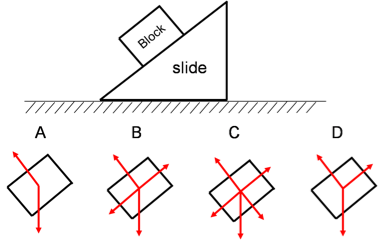
\includegraphics[scale=.4]{/Users/jgates/desktop/latex/pics/incline3.png}
\end{floatingfigure}
 
{\bf \Large{120.}} A block sits at rest and stays at rest on a slide with frictional surfaces. Each red arrow represents a force. Observe their number and direction, but ignore their lengths.  

 \bigskip

\indent Which of the following sketches most closely resembles the correct free body diagram for all forces acting on the block? 

\bigskip 
\vspace{6mm}% Number 130
% CVPMA Algebra Units
% Raptor/BSG drifting apart
% JG

% Watermark
\AddToShipoutPicture*{\BackgroundPic}

\addtocounter {ProbNum} {1}

%\begin{floatingfigure}[r]{.3\textwidth}
%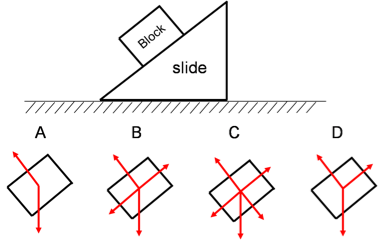
\includegraphics[scale=.4]{/Users/jgates/desktop/latex/pics/incline3.png}
%\end{floatingfigure}
 
{\bf \Large{130.}} Gaeta's Raptor is drifting away from Galactica at a speed of 200 meters per second, while the Galactica drifts away from the Raptor at a speed of 75 meters per second.  The two ships are initially 300 km away from each other.

\bigskip

\indent  How much time will pass before they are 600 km away from each other, and communication is lost?

\bigskip 
\vspace{6mm}% Number 140
% CVPMG Units
% Draw the missing graphs
% JG

% Watermark
\AddToShipoutPicture*{\BackgroundPic}

\addtocounter {ProbNum} {1}

%\begin{floatingfigure}[r]{.3\textwidth}
%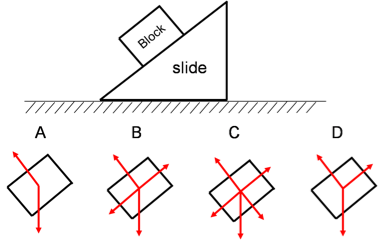
\includegraphics[scale=.4]{/Users/jgates/desktop/latex/pics/incline3.png}
%\end{floatingfigure}
 
{\bf \Large{140.}} Draw the missing graphs.

\bigskip

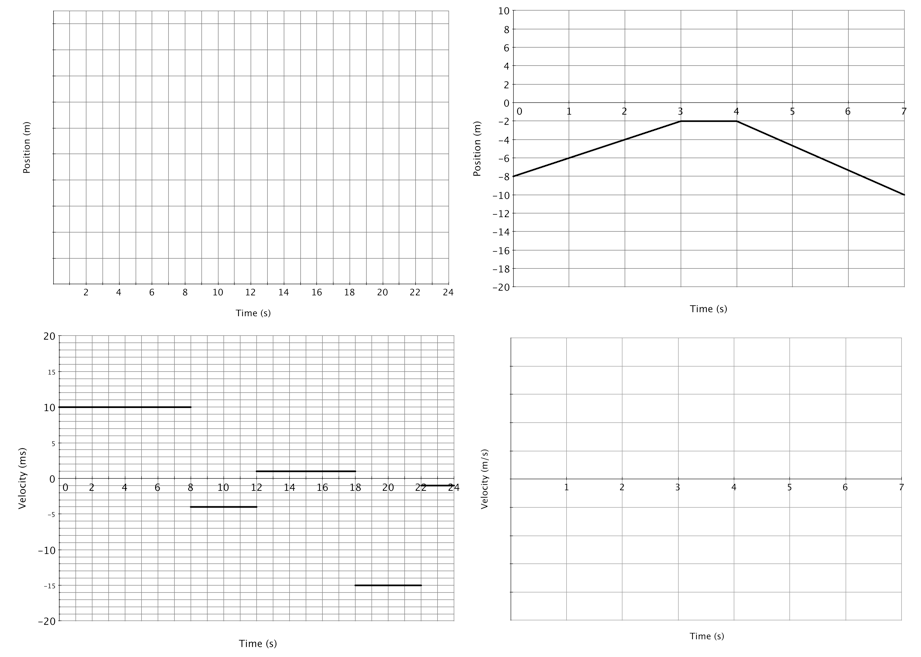
\includegraphics[scale=.57]{/Users/jgates/desktop/latex/pics/cvpmgraphs1.png}

\bigskip 
\vspace{6mm}% Number 150
% CVPMG Units
% Problem-solving, Creed and Kevin on bikes
% JG

% Watermark
\AddToShipoutPicture*{\BackgroundPic}

\addtocounter {ProbNum} {1}

%\begin{floatingfigure}[r]{.3\textwidth}
%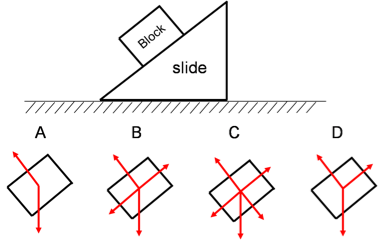
\includegraphics[scale=.4]{/Users/jgates/desktop/latex/pics/incline3.png}
%\end{floatingfigure}
 
{\bf \Large{150.}} Creed and Kevin find some bikes by the loading dock, and devise a competition: they use an 8 meter long rope to tie their bikes together and set up next to each other, facing opposite directions.  They begin next to each other, start their pedaling at the same time and ride in opposite directions, trying to see who can ride the furthest before the rope snaps tight. If Creed can pedal his bike at 4 meters per second, and he ends up 5.1 meters away from the starting point, how fast did Kevin pedal?  Solve it graphically!  Assume that they can get up to speed instantly.

%\bigskip

%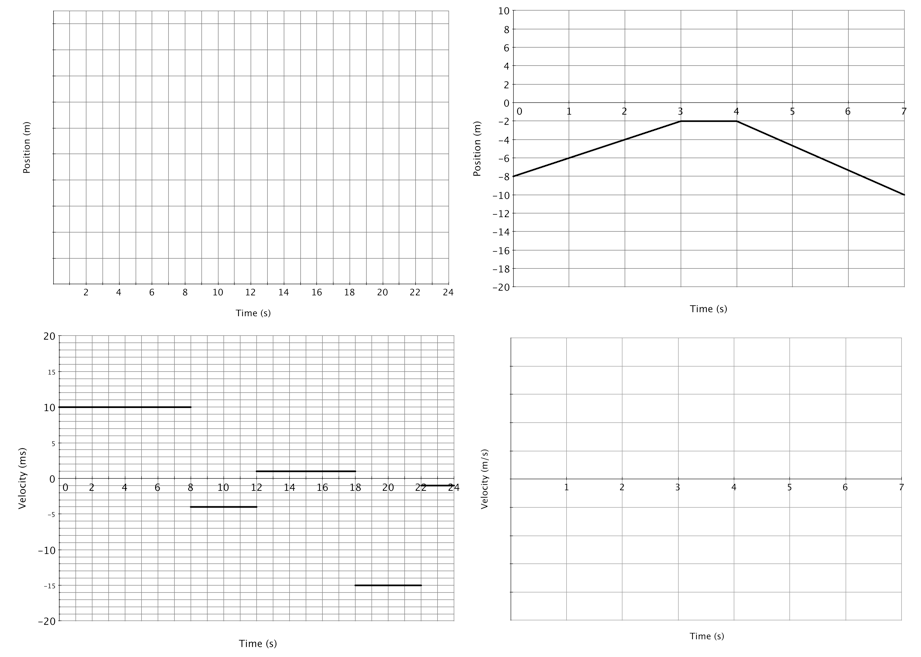
\includegraphics[scale=.57]{/Users/jgates/desktop/latex/pics/cvpmgraphs1.png}

\bigskip 
\vspace{6mm}% Number 160
% CVPMA Units Algebra Prefixes
% Problem-solving, Nostromo signal - hard!
% JG

% Watermark
\AddToShipoutPicture*{\BackgroundPic}

\addtocounter {ProbNum} {1}

%\begin{floatingfigure}[r]{.3\textwidth}
%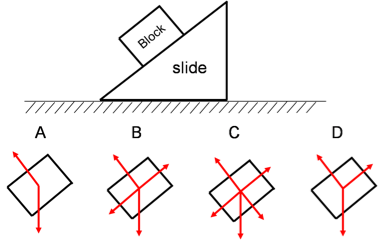
\includegraphics[scale=.4]{/Users/jgates/desktop/latex/pics/incline3.png}
%\end{floatingfigure}
 
{\bf \Large{160.}} As its crew sleeps, the Nostromo glides through space at a brisk clip of ${920~\tfrac{km}{s}}$, relative to a nearby asteroid that it is approaching.  The computer uses radar (object detection using radio waves, which travel at the speed of light: ${3 \times 10^8 ~\tfrac{m}{s}}$) to detect objects in the ship's path.  The radio waves are emitted by the ship, bounce off of the asteroid, and return to the ship, where the computer analyzes the results.

\bigskip
Assume that the asteroid begins at the limit of the ship's effective radar range of 2 million km.  Once it detects the asteroid, the computer will require 15 minutes to revive the crew.  

\bigskip

How much time will the crew have to turn the ship at that point?
%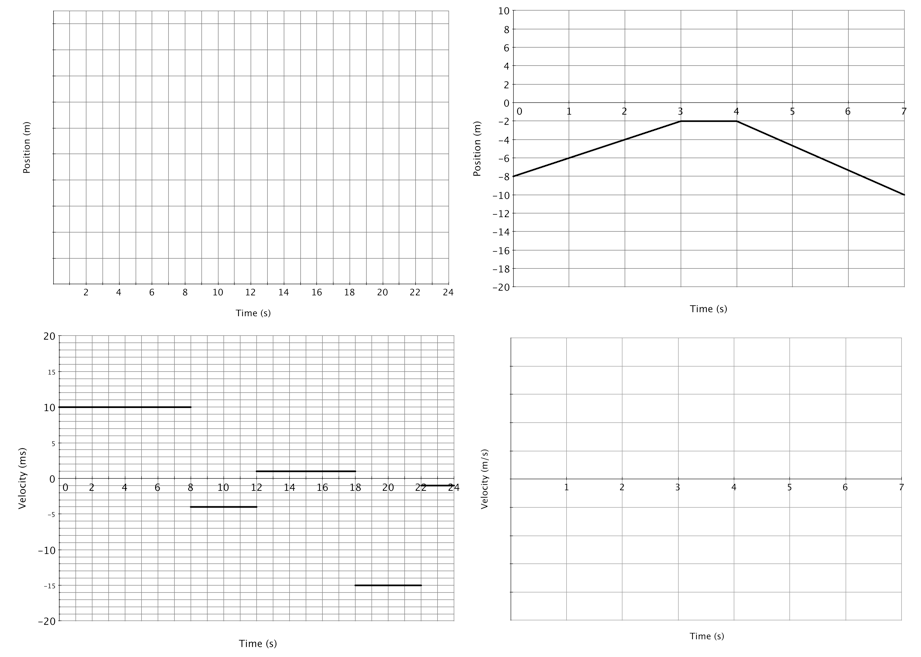
\includegraphics[scale=.57]{/Users/jgates/desktop/latex/pics/cvpmgraphs1.png}

\bigskip 
\vspace{6mm}% Number 160
% CVPMA Algebra Units Prefixes
% Problem-solving, Nostromo signal - hard!
% JG

% Watermark
\AddToShipoutPicture*{\BackgroundPic}

\addtocounter {ProbNum} {1}

%\begin{floatingfigure}[r]{.3\textwidth}
%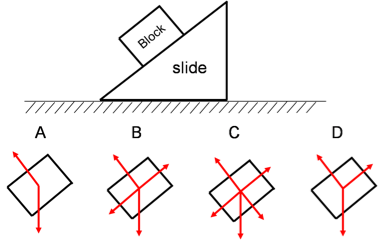
\includegraphics[scale=.4]{/Users/jgates/desktop/latex/pics/incline3.png}
%\end{floatingfigure}
 
{\bf \Large{170.}} As its crew sleeps, the Nostromo glides through space at a brisk clip of ${920~\tfrac{km}{s}}$, relative to a nearby asteroid that it is approaching.  The computer uses radar (object detection using radio waves, which travel at the speed of light: ${3 \times 10^8 ~\tfrac{m}{s}}$) to detect objects in the ship's path.  The radio waves are emitted by the ship, bounce off of the asteroid, and return to the ship, where the computer analyzes the results.

\bigskip
Assume that the asteroid begins at the limit of the ship's effective radar range of 2 million km.  Once it detects the asteroid, the computer will require 15 minutes to revive the crew.  

\bigskip

How much time will the crew have to turn the ship at that point?
%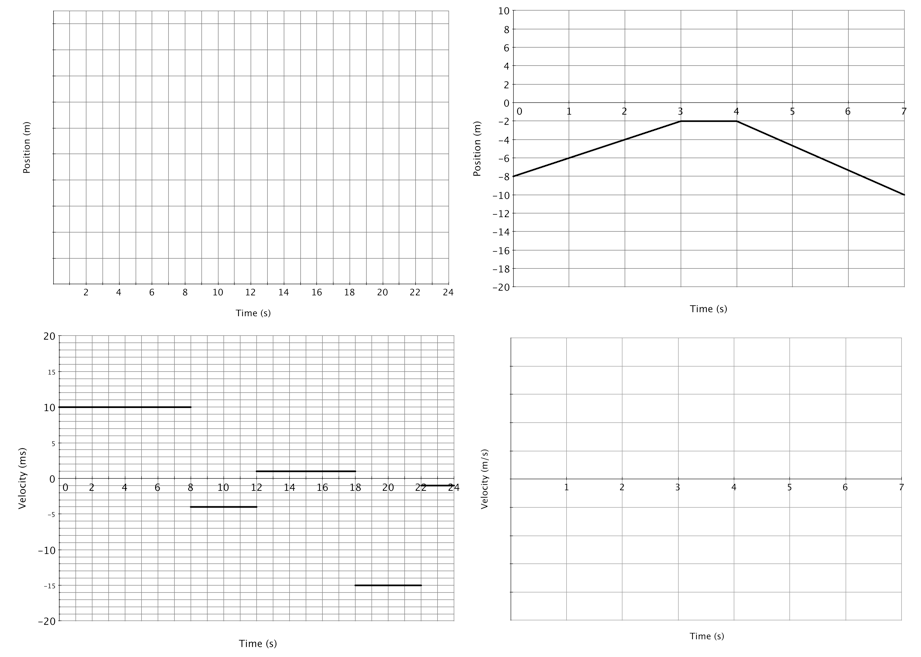
\includegraphics[scale=.57]{/Users/jgates/desktop/latex/pics/cvpmgraphs1.png}

\bigskip 
\vspace{6mm}% Number 180
% CVPMA Algebra Units 
% Problem-solving, RC cars passing each other - hardish
% JG

% Watermark
\AddToShipoutPicture*{\BackgroundPic}

\addtocounter {ProbNum} {1}

%\begin{floatingfigure}[r]{.3\textwidth}
%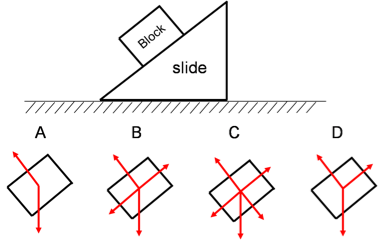
\includegraphics[scale=.4]{/Users/jgates/desktop/latex/pics/incline3.png}
%\end{floatingfigure}
 
{\bf \Large{180.}} A fast RC car (speed: ${12~\tfrac{m}{s}}$ and a slower RC car (${8~\tfrac{m}{s}}$) are 40 meters apart. They then drive directly towards each other.  Some time after the cars have passed each other, the faster car is 15 meters away from the slower one.  

\bigskip

At this moment, how far has the slower one traveled from its starting position? 

%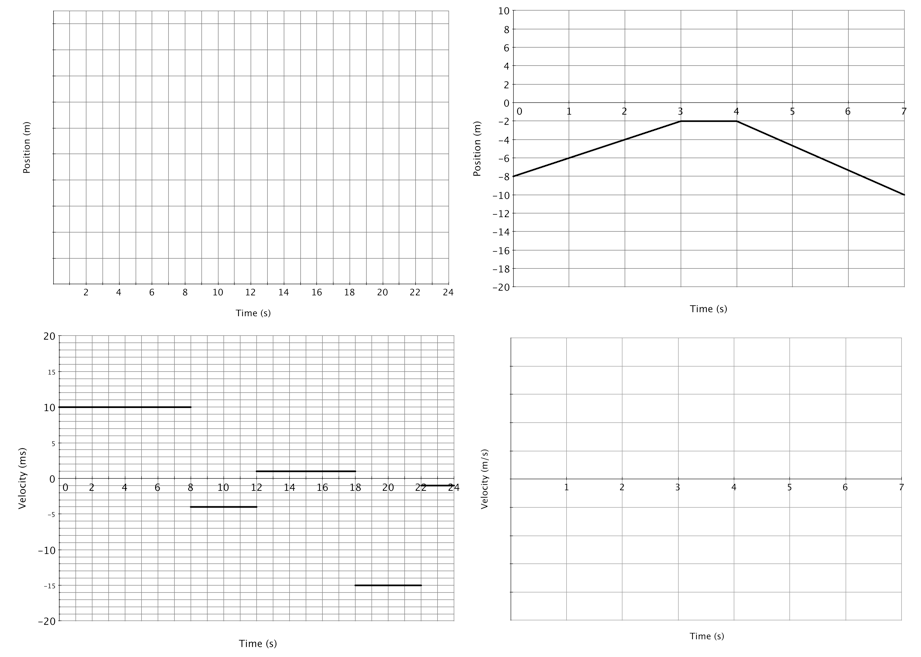
\includegraphics[scale=.57]{/Users/jgates/desktop/latex/pics/cvpmgraphs1.png}

\bigskip 
\vspace{6mm}% Number 190
% CVPMA Algebra Units OddUnits
% Problem-solving, mile marker problem
% Walker

% Watermark
\AddToShipoutPicture*{\BackgroundPic}

\addtocounter {ProbNum} {1}

%\begin{floatingfigure}[r]{.3\textwidth}
%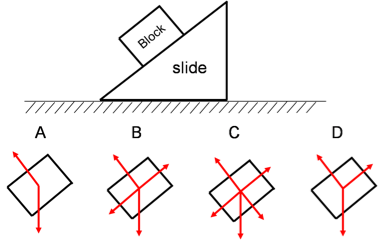
\includegraphics[scale=.4]{/Users/jgates/desktop/latex/pics/incline3.png}
%\end{floatingfigure}
 
{\bf \Large{190.}} You're driving along the highway at constant speed.  When you increase your speed by ${7.9~\tfrac{mi}{hr}}$, the time to go one mile decreases by 13 s. 

\bigskip

What was your original speed?  

%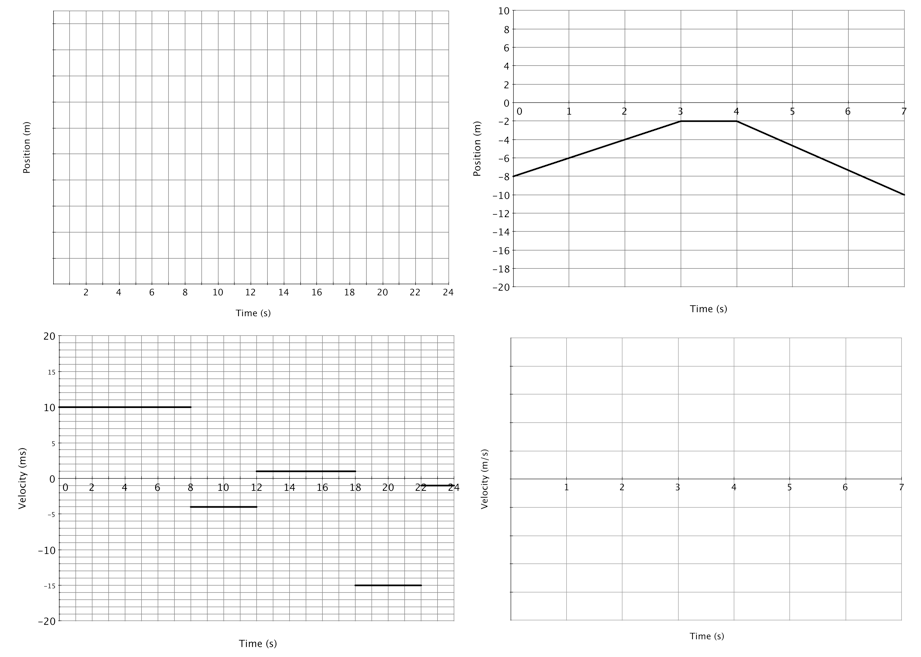
\includegraphics[scale=.57]{/Users/jgates/desktop/latex/pics/cvpmgraphs1.png}

\bigskip 
\vspace{6mm}% Number 20
% UFPM CAPM Friction KFriction 
% Box sliding down frictionless incline: a, motion

% Watermark
\AddToShipoutPicture*{\BackgroundPic}

\addtocounter {ProbNum} {1}

\begin{floatingfigure}[r]{.25\textwidth}
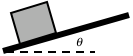
\includegraphics{/Users/jgates/desktop/latex/pics/incline1.png}
\end{floatingfigure} 

{\bf \Large{20.}} A box of mass ${m}$ slides with an initial velocity of ${3~\tfrac{m}{s}}$ down a ramp which is inclined ${20^\circ}$ from the horizontal.  The coefficient of kinetic friction between the ramp and box is .45.

\bigskip

\indent  a. Determine the direction and magnitude of the acceleration of the box as it slides down the incline. 

\bigskip 
b. Discuss the subsequent motion of the box (qualitatively - no numbers are necessary).

\bigskip 
\vspace{6mm}% Number 200
% CVPMG Units
% v to x graph, quantitative
% Walker

% Watermark
\AddToShipoutPicture*{\BackgroundPic}

\addtocounter {ProbNum} {1}

%\begin{floatingfigure}[r]{.3\textwidth}
%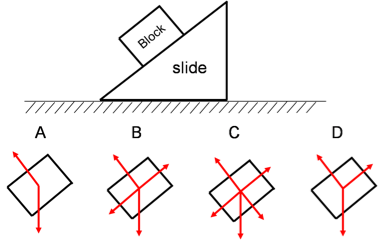
\includegraphics[scale=.4]{/Users/jgates/desktop/latex/pics/incline3.png}
%\end{floatingfigure}
 
{\bf \Large{200.}} Construct a position-vs-time graph for the motion described in the v vs t graph shown below. Assume a position of 10 meters at t = 0. Be sure to number the scale on the position axis.. 

\bigskip

%What was your original speed?  
\begin{center}
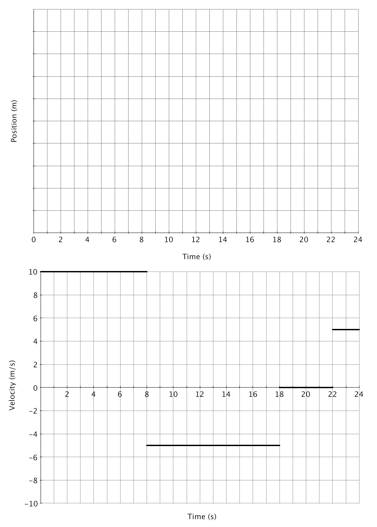
\includegraphics[scale=.77]{/Users/jgates/desktop/latex/pics/vtoxgraph1.png}
\end{center}

\bigskip 
\vspace{6mm}% Number 210
% CVPMA Algebra Units
% Flipper: x modeling given graph
% JG

% Watermark
\AddToShipoutPicture*{\BackgroundPic}

\addtocounter {ProbNum} {1}

\begin{floatingfigure}[r]{.4\textwidth}
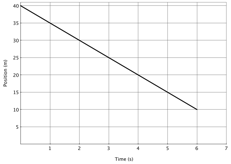
\includegraphics[scale=1]{/Users/jgates/desktop/latex/pics/flipper.png}
\end{floatingfigure}
 
{\bf \Large{210.}} Consider an x vs. t graph for Flipper (you know, the dolphin: king of the sea?).

\bigskip

Agebraically determine Flipper�s position at ${t =}$ 10 s.

%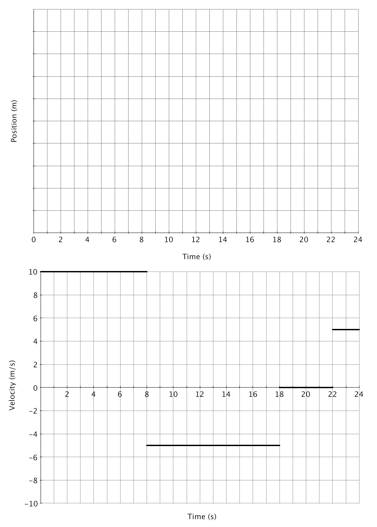
\includegraphics[scale=.77]{/Users/jgates/desktop/latex/pics/vtoxgraph1.png}

\bigskip 
\vspace{6mm}% Number 220
% CVPMG  Units
% Mongooses: avg v/speed, multiple representations
% JG

% Watermark
\AddToShipoutPicture*{\BackgroundPic}

\addtocounter {ProbNum} {1}

%\begin{floatingfigure}[r]{.4\textwidth}
%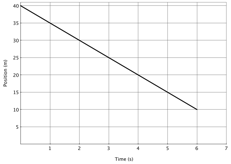
\includegraphics[scale=1]{/Users/jgates/desktop/latex/pics/flipper.png}
%\end{floatingfigure}
 
{\bf \Large{220.}} Two mongooses (mongeese?) walk around on a balance beam:

\begin{center} 
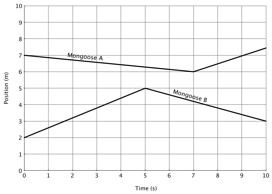
\includegraphics[scale=1]{/Users/jgates/desktop/latex/pics/mongooses.png}
\end{center}

\bigskip
Describe Mongoose A's motion in words.

\bigskip Draw a diagram describing Mongoose B's motion.

\bigskip Which mongoose has the greater average velocity?  Defend your answer.

\bigskip Which mongoose has the greater average speed?  Defend your answer.

\bigskip 
\vspace{6mm}% Number 230
% CVPMG  Units
% Dori/Danica soccer: graphical version
% JG

% Watermark
\AddToShipoutPicture*{\BackgroundPic}

\addtocounter {ProbNum} {1}

%\begin{floatingfigure}[r]{.4\textwidth}
%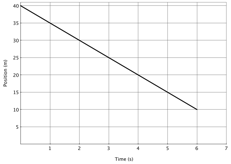
\includegraphics[scale=1]{/Users/jgates/desktop/latex/pics/flipper.png}
%\end{floatingfigure}
 
{\bf \Large{230.}} Dori's running at ${2~\tfrac{m}{s}}$ towards Tower Hill's goal line from 20 meters away when Danica lofts a ball over Dori's head.  The ball hits the ground 3 meters ahead of Dori and rolls towards the goal line at ${4~\tfrac{m}{s}}$.  

\bigskip

It takes 1.5 seconds for Dori to react to the ball; at that point, she begins running faster in order to catch up with the ball before it reaches the goal line.  
%\begin{center} 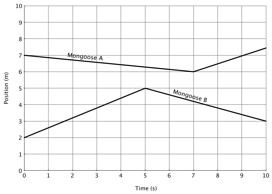
\includegraphics[scale=1]{/Users/jgates/desktop/latex/pics/mongooses.png}
%\end{center}

\bigskip

How fast does she need to run to catch up with the ball before it goes over the goal line? Use graphical problem-solving.

\bigskip 
\vspace{6mm}% Number 231
% CVPMA  Units
% Dori/Danica soccer: algebraic version
% JG

% Watermark
\AddToShipoutPicture*{\BackgroundPic}

\addtocounter {ProbNum} {1}

%\begin{floatingfigure}[r]{.4\textwidth}
%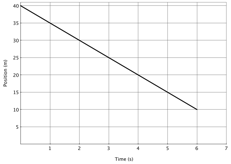
\includegraphics[scale=1]{/Users/jgates/desktop/latex/pics/flipper.png}
%\end{floatingfigure}
 
{\bf \Large{231.}} Dori's running at ${2~\tfrac{m}{s}}$ towards Tower Hill's goal line from 20 meters away when Danica lofts a ball over Dori's head.  The ball hits the ground 3 meters ahead of Dori and rolls towards the goal line at ${4~\tfrac{m}{s}}$.  

\bigskip

It takes 1.5 seconds for Dori to react to the ball; at that point, she begins running faster in order to catch up with the ball before it reaches the goal line.  
%\begin{center} 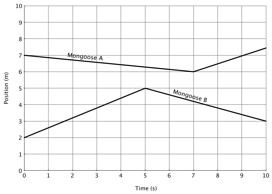
\includegraphics[scale=1]{/Users/jgates/desktop/latex/pics/mongooses.png}
%\end{center}

\bigskip

How fast does she need to run to catch up with the ball before it goes over the goal line? Use algebraic problem-solving.

\bigskip 
\vspace{6mm}% Number 240
% CVPMA Algebra  Units
% Football players running at each other: algebraic version
% JG

% Watermark
\AddToShipoutPicture*{\BackgroundPic}

\addtocounter {ProbNum} {1}

%\begin{floatingfigure}[r]{.4\textwidth}
%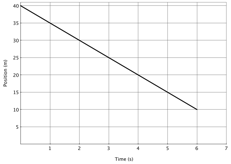
\includegraphics[scale=1]{/Users/jgates/desktop/latex/pics/flipper.png}
%\end{floatingfigure}
 
{\bf \Large{240.}} A running back carries the football down the field, running ${5.6~\tfrac{m}{s}}$.  The slower safety (running speed: ${4.5~\tfrac{m}{s}}$) runs towards him and tries to tackle him. They begin 22 meters apart and run straight at each other.  
%\begin{center} 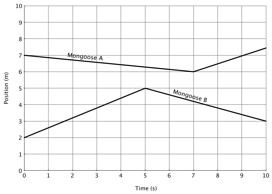
\includegraphics[scale=1]{/Users/jgates/desktop/latex/pics/mongooses.png}
%\end{center}

\bigskip

How far did the running back go before being tackled, and how much time elapsed before he was tackled? Draw a diagram and use algebraic problem solving.

 
\bigskip 
\vspace{6mm}% Number 241
% CVPMG Units
% Football players running at each other: graphical version
% JG

% Watermark
\AddToShipoutPicture*{\BackgroundPic}

\addtocounter {ProbNum} {1}

%\begin{floatingfigure}[r]{.4\textwidth}
%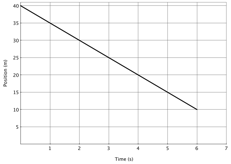
\includegraphics[scale=1]{/Users/jgates/desktop/latex/pics/flipper.png}
%\end{floatingfigure}
 
{\bf \Large{241.}} A running back carries the football down the field, running ${5.6~\tfrac{m}{s}}$.  The slower safety (running speed: ${4.5~\tfrac{m}{s}}$) runs towards him and tries to tackle him. They begin 22 meters apart and run straight at each other.  
%\begin{center} 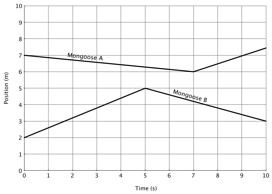
\includegraphics[scale=1]{/Users/jgates/desktop/latex/pics/mongooses.png}
%\end{center}

\bigskip

How far did the running back go before being tackled, and how much time elapsed before he was tackled? Use graphical problem solving.
 
\bigskip 
\vspace{6mm}% Number 250
% CVPMA Algebra Units
% Tron driving at each other
% JG

% Watermark
\AddToShipoutPicture*{\BackgroundPic}

\addtocounter {ProbNum} {1}

%\begin{floatingfigure}[r]{.3\textwidth}
%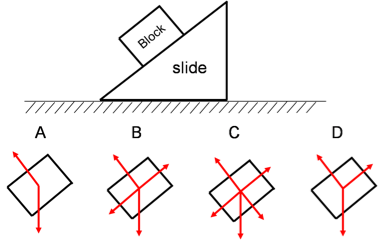
\includegraphics[scale=.4]{/Users/jgates/desktop/latex/pics/incline3.png}
%\end{floatingfigure}
 
{\bf \Large{250.}} Two lightcycles (like from Tron - that movie was awesome, and the remake wasn't bad) charge at each other from an initial distance of 112 meters.  One lightcyle has a constant speed of ${25~\tfrac{m}{s}}$, and the other a constant speed of ${32~\tfrac{m}{s}}$. They drive at each other, barely missing a head-on collision.  

%\begin{center}
%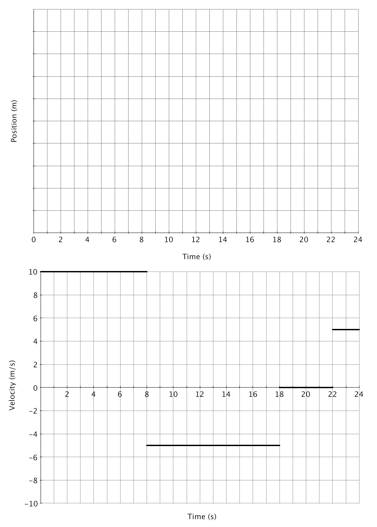
\includegraphics[scale=.77]{/Users/jgates/desktop/latex/pics/vtoxgraph1.png}
%\end{center}

\bigskip
Does CVPM apply? Why or why not?

\bigskip 
How long after they begin driving will they pass each other?
 
\bigskip 
\vspace{6mm}% Number 260
% CVPMA Algebra Units
% Model discrimination, avg v/speed
% JG

% Watermark
\AddToShipoutPicture*{\BackgroundPic}

\addtocounter {ProbNum} {1}

%\begin{floatingfigure}[r]{.3\textwidth}
%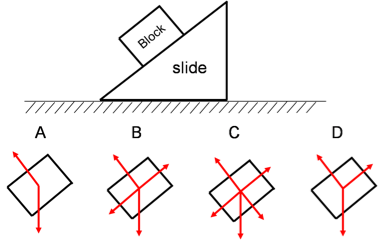
\includegraphics[scale=.4]{/Users/jgates/desktop/latex/pics/incline3.png}
%\end{floatingfigure}
 
{\bf \Large{260.}} A ball is thrown vertically into the air.  It takes 2.42 seconds for it to reach its peak height of 24.5 meters.

\bigskip
Does CVPM apply? Why or why not?

\bigskip 
\bigskip The ball will take another 2.42 seconds to hit the ground.  What is its average velocity over the whole trip?

\bigskip What was the ball's average speed during the whole trip?

%\begin{center}
%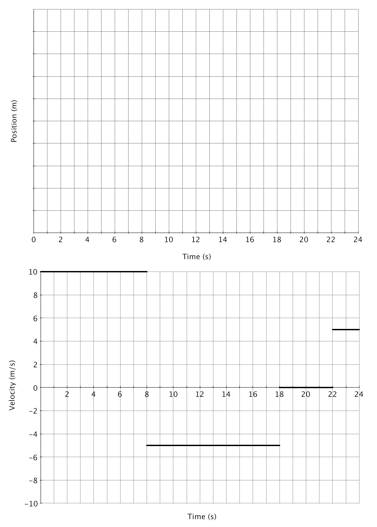
\includegraphics[scale=.77]{/Users/jgates/desktop/latex/pics/vtoxgraph1.png}
%\end{center}
 
\bigskip 
\vspace{6mm}% Number 270
% CVPMA Algebra Units
% Two objects moving, find collision time
% JG

% Watermark
\AddToShipoutPicture*{\BackgroundPic}

\addtocounter {ProbNum} {1}

%\begin{floatingfigure}[r]{.3\textwidth}
%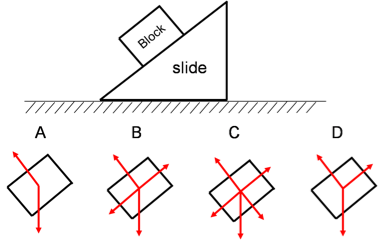
\includegraphics[scale=.4]{/Users/jgates/desktop/latex/pics/incline3.png}
%\end{floatingfigure}
 
{\bf \Large{270.}} Instead of waiting for a soccer pass to come to you, moving towards the ball can greatly increase your chances of not having the ball stolen.  A pass is made to you from 25 meters away, with a speed of ${13~\tfrac{m}{s}}$.  After a .4 second pause (your reaction time), you begin running towards the ball at ${5~\tfrac{m}{s}}$.

\bigskip
What issues might make a CVPM model of this situation less than faithful to the real situation?

\vspace{30mm}
Where (at what position) will you receive the pass?

%\begin{center}
%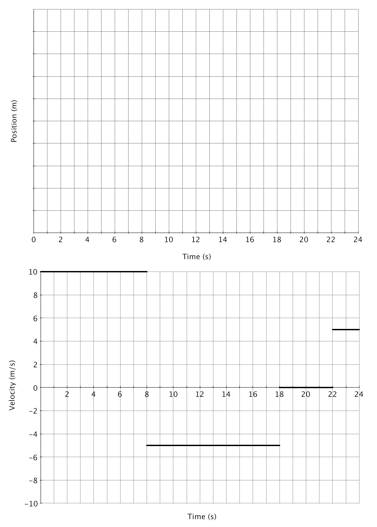
\includegraphics[scale=.77]{/Users/jgates/desktop/latex/pics/vtoxgraph1.png}
%\end{center}
 
\bigskip 
\vspace{6mm}% Number 271
% CVPMG Units
% Two objects moving, find collision time, graphical version
% JG

% Watermark
\AddToShipoutPicture*{\BackgroundPic}

\addtocounter {ProbNum} {1}

%\begin{floatingfigure}[r]{.3\textwidth}
%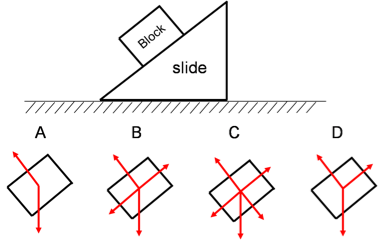
\includegraphics[scale=.4]{/Users/jgates/desktop/latex/pics/incline3.png}
%\end{floatingfigure}
 
{\bf \Large{271.}} Instead of waiting for a soccer pass to come to you, moving towards the ball can greatly increase your chances of not having the ball stolen.  A pass is made to you from 25 meters away, with a speed of ${13~\tfrac{m}{s}}$.  After a .4 second pause (your reaction time), you begin running towards the ball at ${5~\tfrac{m}{s}}$.

\bigskip
What issues might make a CVPM model of this situation less than faithful to the real situation?

\vspace{30mm}
Where (at what position) will you receive the pass? Use graphical problem-solving.

%\begin{center}
%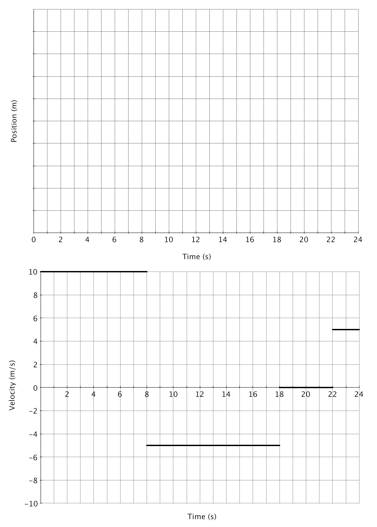
\includegraphics[scale=.77]{/Users/jgates/desktop/latex/pics/vtoxgraph1.png}
%\end{center}
 
\bigskip 
\vspace{6mm}% Number 280
% CVPMA Algebra Units
% Dune buggy overtaking, find distance
% JG

% Watermark
\AddToShipoutPicture*{\BackgroundPic}

\addtocounter {ProbNum} {1}

%\begin{floatingfigure}[r]{.3\textwidth}
%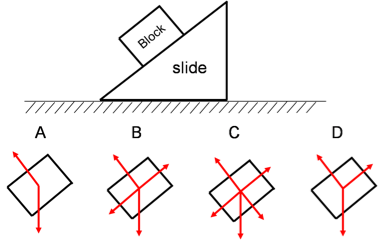
\includegraphics[scale=.4]{/Users/jgates/desktop/latex/pics/incline3.png}
%\end{floatingfigure}
 
{\bf \Large{280.}}A dune buggy takes off down the beach, driving ${8.9~\tfrac{m}{s}}$.  It then passes a second dune buggy, which sets off after it at a speed of ${12.1~\tfrac{m}{s}}$, after waiting four seconds to start.

\bigskip
Describe some ways in which a CVPM model of this situation would not match reality.

\bigskip How far has the first dune buggy traveled when it is caught by the second dune buggy?

%\begin{center}
%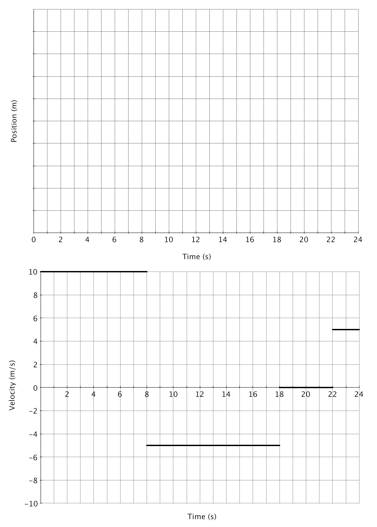
\includegraphics[scale=.77]{/Users/jgates/desktop/latex/pics/vtoxgraph1.png}
%\end{center}
 
\bigskip 
\vspace{6mm}% Number 281
% CVPMA Algebra Units
% Dune buggy overtaking, find time
% JG

% Watermark
\AddToShipoutPicture*{\BackgroundPic}

\addtocounter {ProbNum} {1}

%\begin{floatingfigure}[r]{.3\textwidth}
%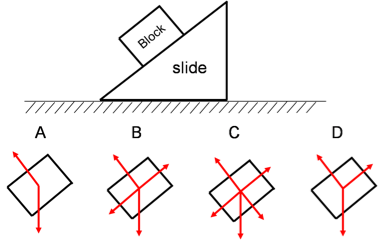
\includegraphics[scale=.4]{/Users/jgates/desktop/latex/pics/incline3.png}
%\end{floatingfigure}
 
{\bf \Large{281.}}A dune buggy takes off down the beach, driving ${8.9~\tfrac{m}{s}}$.  It then passes a second dune buggy, which sets off after it at a speed of ${12.1~\tfrac{m}{s}}$, after waiting four seconds to start.

\bigskip
Describe some ways in which a CVPM model of this situation would not match reality.

\bigskip For how long has the first dune buggy traveled when it is caught by the second dune buggy?

%\begin{center}
%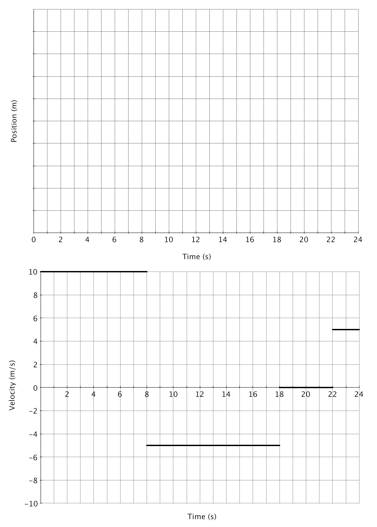
\includegraphics[scale=.77]{/Users/jgates/desktop/latex/pics/vtoxgraph1.png}
%\end{center}
 
\bigskip 
\vspace{6mm}% Number 290
% CVPMA Algebra Units
% Avg. v, speed, dsiplacement
% JG

% Watermark
\AddToShipoutPicture*{\BackgroundPic}

\addtocounter {ProbNum} {1}

%\begin{floatingfigure}[r]{.3\textwidth}
%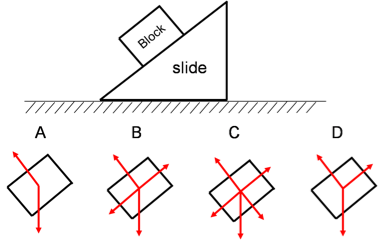
\includegraphics[scale=.4]{/Users/jgates/desktop/latex/pics/incline3.png}
%\end{floatingfigure}
 
{\bf \Large{290.}}A squirrel runs back and forth on a fence rail.  It runs east 4 meters in 1.2 seconds, then pauses for .8 seconds, then runs west 6 meters in 1.3 seconds, and then east 7 meters in 4 seconds.

\bigskip
What was the squirrel's maximum speed?

\bigskip 
\bigskip \bigskip What was the squirrel's displacement during the first 3 seconds?
 
%\begin{center}
%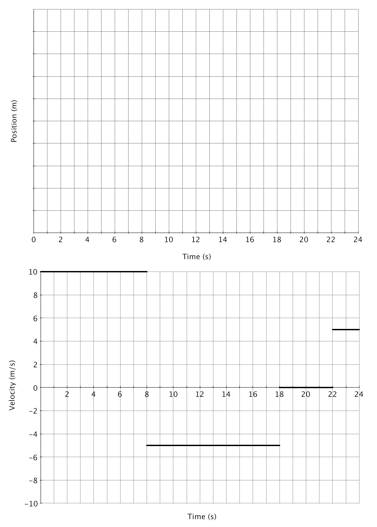
\includegraphics[scale=.77]{/Users/jgates/desktop/latex/pics/vtoxgraph1.png}
%\end{center}
 
\bigskip 
\vspace{6mm}% Number 30
% Algebra
% Number of coins - algebra problem
% MIT Physics for Teachers LON-CAPA

% Watermark
\AddToShipoutPicture*{\BackgroundPic}

\addtocounter {ProbNum} {1}

%\begin{floatingfigure}[r]{.2\textwidth}
%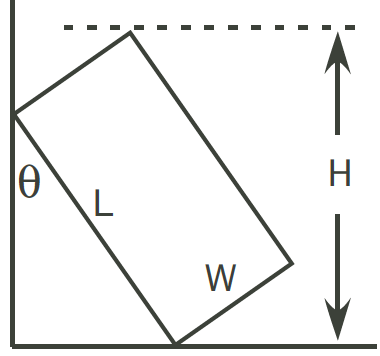
\includegraphics[scale=1]{/Users/jgates/desktop/latex/pics/leaningbox.png}
%\end{floatingfigure}
 
{\bf \Large{30.}} Britney has 25 coins, all nickels (5 cents) and dimes (10 cents). If the nickels were changed to quarters (25 cents) and the dimes changed to nickels, the total value of the coins would remain unchanged. 

\bigskip

\indent How many nickels and how many dimes does she have? 

\bigskip 
\vspace{6mm}% Number 300
% CVPMG Algebra Units
% Avg. v, speed, displacement, graph conversion
% JG

% Watermark
\AddToShipoutPicture*{\BackgroundPic}

\addtocounter {ProbNum} {1}

%\begin{floatingfigure}[r]{.3\textwidth}
%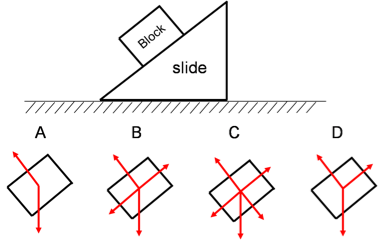
\includegraphics[scale=.4]{/Users/jgates/desktop/latex/pics/incline3.png}
%\end{floatingfigure}
 
{\bf \Large{300.}}Draw the corresponding motion graphs.

\begin{center}
\includegraphics[scale=.77]{/Users/jgates/desktop/latex/pics/cvpmgraphs2.png}
\end{center}

\bigskip
Which motion has the greater (magnitude of) displacement?
 
\bigskip Which motion has the greater (magnitude of) average velocity?

\bigskip Which motion has the greater average speed?

\bigskip Which motion has the greater distance traveled?

\bigskip 
\vspace{6mm}% Number 310
% CVPMG  Units
% Graph description, problem-solving
% JG

% Watermark
\AddToShipoutPicture*{\BackgroundPic}

\addtocounter {ProbNum} {1}

%\begin{floatingfigure}[r]{.3\textwidth}
%\includegraphics[scale=.4]{/Users/jgates/desktop/latex/pics/incline3.png}
%\end{floatingfigure}
 
{\bf \Large{310.}}An exciting chase has broken out between a toy police car and a toy speeder (running from the police because he foolishly doesn�t have any toy insurance).  
 
\begin{center}
\includegraphics[scale=.87]{/Users/jgates/desktop/latex/pics/cvpm2.png}
\end{center}

\bigskip
Describe the segment of the chase shown so far, as accurately as you can (ie: including exact values).
 
\bigskip Assuming that the toy police car can get up to speed very quickly, how fast will it need to go in order to catch the speeder before ${t=~}$20 s?

\bigskip 
\vspace{6mm}% Number 320
% CVPMG Units
% Chase after distance pause: problem-solving
% JG

% Watermark
\AddToShipoutPicture*{\BackgroundPic}

\addtocounter {ProbNum} {1}

%\begin{floatingfigure}[r]{.3\textwidth}
%\includegraphics[scale=.4]{/Users/jgates/desktop/latex/pics/incline3.png}
%\end{floatingfigure}
 
{\bf \Large{320.}}A real police car chases down a stolen sturgeon truck.  The police car is sitting by the side of the road when the truck flies by at ${35~\tfrac{m}{s}}$.  Assume that the police officer reacts after the truck is 150 meters past her and gets up to speed instantly.  
 
%\begin{center}
%\includegraphics[scale=.87]{/Users/jgates/desktop/latex/pics/cvpm2.png}
%\end{center}

\bigskip
How fast does she need to go in order to catch the truck within 2 minutes? Use graphical problem-solving.
 
\bigskip 
\vspace{6mm}% Number 321
% CVPMA Algebra Units
% Chase after distance pause: problem-solving
% JG

% Watermark
\AddToShipoutPicture*{\BackgroundPic}

\addtocounter {ProbNum} {1}

%\begin{floatingfigure}[r]{.3\textwidth}
%\includegraphics[scale=.4]{/Users/jgates/desktop/latex/pics/incline3.png}
%\end{floatingfigure}
 
{\bf \Large{321.}}A real police car chases down a stolen sturgeon truck.  The police car is sitting by the side of the road when the truck flies by at ${35~\tfrac{m}{s}}$.  Assume that the police officer reacts after the truck is 150 meters past her and gets up to speed instantly.  
 
%\begin{center}
%\includegraphics[scale=.87]{/Users/jgates/desktop/latex/pics/cvpm2.png}
%\end{center}

\bigskip
How fast does she need to go in order to catch the truck within 2 minutes? Use algebraic problem-solving.
 
\bigskip 
\vspace{6mm}% Number 325
% CVPMA Algebra Units
% Chase after time pause: problem-solving
% JG

% Watermark
\AddToShipoutPicture*{\BackgroundPic}

\addtocounter {ProbNum} {1}

%\begin{floatingfigure}[r]{.3\textwidth}
%\includegraphics[scale=.4]{/Users/jgates/desktop/latex/pics/incline3.png}
%\end{floatingfigure}
 
{\bf \Large{325.}}A real police car chases down a stolen sturgeon truck.  The police car is sitting by the side of the road when the truck flies by at ${35~\tfrac{m}{s}}$.  The police officer takes 1.5 seconds to react, but we'll assume that she can get the car up to speed instantly.

%\begin{center}
%\includegraphics[scale=.87]{/Users/jgates/desktop/latex/pics/cvpm2.png}
%\end{center}

\bigskip
how fast will she have to go in order to catch the speeder within 2 km? Use algebraic problem-solving.
 
\bigskip 
\vspace{6mm}% Number 326
% CVPMG Units
% Chase after time pause: problem-solving, assumption
% JG

% Watermark
\AddToShipoutPicture*{\BackgroundPic}

\addtocounter {ProbNum} {1}

%\begin{floatingfigure}[r]{.3\textwidth}
%\includegraphics[scale=.4]{/Users/jgates/desktop/latex/pics/incline3.png}
%\end{floatingfigure}
 
{\bf \Large{326.}}A real police car chases down a stolen sturgeon truck.  The police car is sitting by the side of the road when the truck flies by at ${35~\tfrac{m}{s}}$.  The police officer takes 1.5 seconds to react, but we'll assume that she can get the car up to speed instantly.

%\begin{center}
%\includegraphics[scale=.87]{/Users/jgates/desktop/latex/pics/cvpm2.png}
%\end{center}

\bigskip
How fast will she have to go in order to catch the speeder within 2 km? Use graphical problem-solving.
 
\bigskip Graph (with a dotted line for the police car, but on the same axes as before) a more realistic scenario, where she requires time to get up to full speed.

\bigskip

What will this do to the top speed that will be required to catch the truck within 2 km?  Make sure that your graph agrees with this!
\bigskip \vspace{6mm}% Number 330
% CAPMG Units
% Graph conversion x->v->a
% JG

% Watermark
\AddToShipoutPicture*{\BackgroundPic}

\addtocounter {ProbNum} {1}

%\begin{floatingfigure}[r]{.3\textwidth}
%\includegraphics[scale=.4]{/Users/jgates/desktop/latex/pics/incline3.png}
%\end{floatingfigure}
 
{\bf \Large{330.}} Draw the velocity and acceleration graphs that correspond to the given position graph.

\begin{center}
\includegraphics[scale=1]{/Users/jgates/desktop/latex/pics/givenxgraph1.png}
\end{center}

\begin{center}
\includegraphics[scale=1]{/Users/jgates/desktop/latex/pics/blankvgraph1.png}
\end{center}

\begin{center}
\includegraphics[scale=1]{/Users/jgates/desktop/latex/pics/blankagraph1.png}
\end{center}


\bigskip \vspace{6mm}% Number 340
% CAPMG Units
% Graph conversion a->v->x
% JG

% Watermark
\AddToShipoutPicture*{\BackgroundPic}

\addtocounter {ProbNum} {1}

%\begin{floatingfigure}[r]{.3\textwidth}
%\includegraphics[scale=.4]{/Users/jgates/desktop/latex/pics/incline3.png}
%\end{floatingfigure}
 
{\bf \Large{340.}} Draw the position and velocity graphs that correspond to the given acceleration graph, initial position of -3 meters, and initial velocity of ${2~\tfrac{m}{s}}$.

\begin{center}
\includegraphics[scale=1]{/Users/jgates/desktop/latex/pics/blankxgraph2.png}
\end{center}

\begin{center}
\includegraphics[scale=1]{/Users/jgates/desktop/latex/pics/blankvgraph2.png}
\end{center}

\begin{center}
\includegraphics[scale=1]{/Users/jgates/desktop/latex/pics/givenagraph2.png}
\end{center}


\bigskip \vspace{6mm}% Number 350
% CAPMA Algebra Units
% Car slowing up hill
% JG

% Watermark
\AddToShipoutPicture*{\BackgroundPic}

\addtocounter {ProbNum} {1}

%\begin{floatingfigure}[r]{.3\textwidth}
%\includegraphics[scale=.4]{/Users/jgates/desktop/latex/pics/incline3.png}
%\end{floatingfigure}
 
{\bf \Large{350.}} A car that is moving ${30~\tfrac{m}{s}}$ runs out of gas while driving up a hill.  The car comes to a stop 150 meters further up the hill than the point at which it ran out of gas. 

\begin{center}
\includegraphics[scale=.6]{/Users/jgates/desktop/latex/pics/caruphill.png}
\end{center}

\bigskip  How long, after running out of gas, did it take for the car to come to a stop?  Also describe, in words, the direction of the acceleration. Draw a kinematics diagram as part of your solution.


\bigskip \vspace{6mm}% Number 360
% CAPMG 
% Token toss - qual graph stack describing motion, avg v
% JG

% Watermark
\AddToShipoutPicture*{\BackgroundPic}

\addtocounter {ProbNum} {1}

\begin{floatingfigure}[r]{.15\textwidth}
\includegraphics[scale=.8]{/Users/jgates/desktop/latex/pics/tokentoss.png}
\end{floatingfigure}
 
{\bf \Large{360.}} A man, on the ground, throws a subway token to his friend on the platform above.  The token is thrown essentially straight up; it flies past the friend and falls back to him. Call the lower man�s hand ${y=0}$ and define �up� as positive.

\bigskip  Draw graphs of the token�s vertical position, velocity, and acceleration during the trip.  No numbers are necessary.
Make sure that the time scales of the three graphs line up.

\begin{center}
\includegraphics[scale=.85]{/Users/jgates/desktop/latex/pics/blankyvagraphstack.png}
\end{center}

\bigskip Finally, show on both the position and velocity graphs the \emph sign (is it positive, negative, or zero?) of the average velocity for the trip.  Be sure that it�s clear which characteristic of each graph you used to determine the sign of the average velocity!

\bigskip \vspace{6mm}% Number 370
% CAPMA Algebra Units
% Cannon shot straight up - how much time? Graphical
% JG

% Watermark
\AddToShipoutPicture*{\BackgroundPic}

\addtocounter {ProbNum} {1}

%\begin{floatingfigure}[r]{.15\textwidth}
%\includegraphics[scale=.8]{/Users/jgates/desktop/latex/pics/tokentoss.png}
%\end{floatingfigure}
 
{\bf \Large{370.}} A cannon is shot straight up into the air. The cannonball leaves the cannon moving ${45~\tfrac{m}{s}}$.  

\bigskip  After how much time in the air will it have a speed of ${20~\tfrac{m}{s}}$? 

%\begin{center}
%\includegraphics[scale=.85]{/Users/jgates/desktop/latex/pics/blankyvagraphstack.png}
%\end{center}


\bigskip \vspace{6mm}% Number 371
% CAPMG Units
% Cannon shot straight up - how much time? Graphical
% JG

% Watermark
\AddToShipoutPicture*{\BackgroundPic}

\addtocounter {ProbNum} {1}

%\begin{floatingfigure}[r]{.15\textwidth}
%\includegraphics[scale=.8]{/Users/jgates/desktop/latex/pics/tokentoss.png}
%\end{floatingfigure}
 
{\bf \Large{371.}} A cannon is shot straight up into the air. The cannonball leaves the cannon moving ${45~\tfrac{m}{s}}$.  

\bigskip  After how much time in the air will it have a speed of ${20~\tfrac{m}{s}}$? Use graphical problem-solving.

%\begin{center}
%\includegraphics[scale=.85]{/Users/jgates/desktop/latex/pics/blankyvagraphstack.png}
%\end{center}


\bigskip \vspace{6mm}% Number 372
% CAPMA Algebra Units
% Cannon shot straight up - how much time? Algebraic
% JG

% Watermark
\AddToShipoutPicture*{\BackgroundPic}

\addtocounter {ProbNum} {1}

%\begin{floatingfigure}[r]{.15\textwidth}
%\includegraphics[scale=.8]{/Users/jgates/desktop/latex/pics/tokentoss.png}
%\end{floatingfigure}
 
{\bf \Large{372.}} A cannon is shot straight up into the air. The cannonball leaves the cannon moving ${45~\tfrac{m}{s}}$.  

\bigskip  After how much time in the air will it have a speed of ${20~\tfrac{m}{s}}$? Use algebraic problem-solving.

%\begin{center}
%\includegraphics[scale=.85]{/Users/jgates/desktop/latex/pics/blankyvagraphstack.png}
%\end{center}


\bigskip \vspace{6mm}% Number 380
% CAPM
% Skateboarder jump a direction determination
% JG

% Watermark
\AddToShipoutPicture*{\BackgroundPic}

\addtocounter {ProbNum} {1}

%\begin{floatingfigure}[r]{.15\textwidth}
%\includegraphics[scale=.8]{/Users/jgates/desktop/latex/pics/tokentoss.png}
%\end{floatingfigure}
 
{\bf \Large{380.}} A diagram of a crazy skateboarder's stunt is shown below.  The skateboarder begins at rest at the top of the ramp, goes down the ramp, up the small ramp, and flies off of the ramp.  Do the following:


\MakeList{a.}{
\item Draw and label acceleration vectors for sections A, B, and C.  That�s three vectors to draw. 
\item Draw and label initial and final velocity vectors for sections A and B -- that's four more vectors to draw.  Place the tails of these vectors at the ends of the dotted segments denoting the three sections.  Make their lengths proportionate to the speeds. 
}

\begin{center}
\includegraphics[scale=.85]{/Users/jgates/desktop/latex/pics/blankyvagraphstack.png}
\end{center}


\bigskip \vspace{6mm}% Number 390
% CAPM Algebra Units
% Meteor chunk slowdown
% JG

% Watermark
\AddToShipoutPicture*{\BackgroundPic}

\addtocounter {ProbNum} {1}

%\begin{floatingfigure}[r]{.15\textwidth}
%\includegraphics[scale=.8]{/Users/jgates/desktop/latex/pics/tokentoss.png}
%\end{floatingfigure}
 
{\bf \Large{390.}} A rock fragment is traveling ${640~\tfrac{m}{s}}$  when it is knocked off of a falling meteor. It has slowed to ${590~\tfrac{m}{s}}$  after .6 seconds.  Assume a constant acceleration. 

\bigskip
How far will it have gone after 2 seconds? 

%\begin{center}
%\includegraphics[scale=.85]{/Users/jgates/desktop/latex/pics/blankyvagraphstack.png}
%\end{center}


\bigskip \vspace{6mm}% Number 391
% CAPMA Algebra Units
% Meteor chunk slowdown; algebraic version
% JG

% Watermark
\AddToShipoutPicture*{\BackgroundPic}

\addtocounter {ProbNum} {1}

%\begin{floatingfigure}[r]{.15\textwidth}
%\includegraphics[scale=.8]{/Users/jgates/desktop/latex/pics/tokentoss.png}
%\end{floatingfigure}
 
{\bf \Large{391.}} A rock fragment is traveling ${640~\tfrac{m}{s}}$  when it is knocked off of a falling meteor. It has slowed to ${590~\tfrac{m}{s}}$  after .6 seconds.  Assume a constant acceleration. 

\bigskip
How far will it have gone after 2 seconds? Use algebraic problem-solving.

%\begin{center}
%\includegraphics[scale=.85]{/Users/jgates/desktop/latex/pics/blankyvagraphstack.png}
%\end{center}


\bigskip \vspace{6mm}% Number 392
% CAPMG  Units
% Meteor chunk slowdown; algebraic version
% JG

% Watermark
\AddToShipoutPicture*{\BackgroundPic}

\addtocounter {ProbNum} {1}

%\begin{floatingfigure}[r]{.15\textwidth}
%\includegraphics[scale=.8]{/Users/jgates/desktop/latex/pics/tokentoss.png}
%\end{floatingfigure}
 
{\bf \Large{392.}} A rock fragment is traveling ${640~\tfrac{m}{s}}$  when it is knocked off of a falling meteor. It has slowed to ${590~\tfrac{m}{s}}$  after .6 seconds.  Assume a constant acceleration. 

\bigskip
How far will it have gone after 2 seconds? Use graphical problem-solving.

%\begin{center}
%\includegraphics[scale=.85]{/Users/jgates/desktop/latex/pics/blankyvagraphstack.png}
%\end{center}


\bigskip \vspace{6mm}% Number 40
% Algebra
% Quartic equation solving algebra problem
% MIT Physics for Teachers LON-CAPA

% Watermark
\AddToShipoutPicture*{\BackgroundPic}

\addtocounter {ProbNum} {1}

%\begin{floatingfigure}[r]{.2\textwidth}
%\includegraphics[scale=1]{/Users/jgates/desktop/latex/pics/leaningbox.png}
%\end{floatingfigure}
 
{\bf \Large{40.}} Find all possible values of $x$ which solve the equation ${x^{4}-20\cdot x^{2}+64=0}$.

%\bigskip

%\indent How many nickels and how many dimes does she have? 

\bigskip 
\vspace{6mm}% Number 400
% UFPM
% Airplane climb Fnet direction
% MIT

% Watermark
\AddToShipoutPicture*{\BackgroundPic}

\addtocounter {ProbNum} {1}

\begin{floatingfigure}[r]{.35\textwidth}
\includegraphics[scale=.5]{/Users/jgates/desktop/latex/pics/airplaneclimb.png}
\end{floatingfigure}
 
{\bf \Large{400.}} An airplane is gaining height as indicated. The airplane is slowing down.

\bigskip
Which of these vectors could be the direction of the net force on a passenger in the plane? Explain!

\setlength{\unitlength}{1mm}
\begin{picture}(100, 40)
  \thicklines
  \put(20, 20){\vector(-2, 1){20}}
  \put(30, 30){\vector(2, -1){20}}
  \put(65, 35){\vector(0, -2){20}}
  \put(95, 35){\vector(-1, -2){10}}
\end{picture}


%\begin{center}
%\includegraphics[scale=.85]{/Users/jgates/desktop/latex/pics/blankyvagraphstack.png}
%\end{center}


\bigskip \vspace{6mm}% Number 410
% StaticEq
% Hanging sign
% MIT

% Watermark
\AddToShipoutPicture*{\BackgroundPic}

\addtocounter {ProbNum} {1}

\begin{floatingfigure}[r]{.35\textwidth}
\includegraphics[scale=.5]{/Users/jgates/desktop/latex/pics/staticeq1.png}
\end{floatingfigure}
 
{\bf \Large{410.}} A sign is supported by a horizontal beam and a diagonal wire as shown, both attached to a wall. The sign has a mass $m$, which is very large compared to the mass of the wire and the beam (i.e., neglect the mass of the wire and the beam). The beam pivots freely around its anchoring point in the wall, so it provides no support in the vertical direction. The angle between the wire and the beam is $\varphi$. 

\bigskip
Determine the magnitude of the force exerted by the beam.

%\begin{center}
%\includegraphics[scale=.85]{/Users/jgates/desktop/latex/pics/blankyvagraphstack.png}
%\end{center}


\bigskip \vspace{6mm}% Number 420
% StaticEq
% Teeter totter
% MIT

% Watermark
\AddToShipoutPicture*{\BackgroundPic}

\addtocounter {ProbNum} {1}

\begin{floatingfigure}[r]{.35\textwidth}
\includegraphics[scale=.5]{/Users/jgates/desktop/latex/pics/staticeq1.png}
\end{floatingfigure}
 
{\bf \Large{420.}} A long uniform board weighs 57.7 N (11.5 lbs) rests on a support at its mid point. Two children weighing 401.0 N (80.2 lbs) and 470.0 N (94.0 lbs) stand on the board so that the board is balanced. 

\bigskip
What is the upward force exerted on the board by the support? 

%\begin{center}
%\includegraphics[scale=.85]{/Users/jgates/desktop/latex/pics/blankyvagraphstack.png}
%\end{center}


\bigskip \vspace{6mm}% Number 430
% StaticEq
% Hammock static eq -hard
% MIT

% Watermark
\AddToShipoutPicture*{\BackgroundPic}

\addtocounter {ProbNum} {1}

%\begin{floatingfigure}[r]{.35\textwidth}
%\includegraphics[scale=.5]{/Users/jgates/desktop/latex/pics/staticeq1.png}
%\end{floatingfigure}
 
{\bf \Large{430.}} Your friend of mass ${m}$ sits in a hammock that is centered between two vertical posts separated by a distance ${d}$. The hammock dips a distance ${h}$ below the height at which the hammock is secured to the posts. 

\bigskip
What is the horizontal force on each post due to your friend? 

%\begin{center}
%\includegraphics[scale=.85]{/Users/jgates/desktop/latex/pics/blankyvagraphstack.png}
%\end{center}


\bigskip \vspace{6mm}% Number 440
% UFPM Tension
% pulling mass up with string - easy
% MIT

% Watermark
\AddToShipoutPicture*{\BackgroundPic}

\addtocounter {ProbNum} {1}

%\begin{floatingfigure}[r]{.35\textwidth}
%\includegraphics[scale=.5]{/Users/jgates/desktop/latex/pics/staticeq1.png}
%\end{floatingfigure}
 
{\bf \Large{440.}} A 2.45 kg mass is suspended from a string which is pulled upward. The mass accelerates upwards with an acceleration of ${2.3~\tfrac{m}{s^2}}$. 
\bigskip
What is the tension in the string?

%\begin{center}
%\includegraphics[scale=.85]{/Users/jgates/desktop/latex/pics/blankyvagraphstack.png}
%\end{center}


\bigskip \vspace{6mm}% Number 450
% BFPM Springs
% Spring holding object at rest - a bit tricky with length
% MIT

% Watermark
\AddToShipoutPicture*{\BackgroundPic}

\addtocounter {ProbNum} {1}

%\begin{floatingfigure}[r]{.35\textwidth}
%\includegraphics[scale=.5]{/Users/jgates/desktop/latex/pics/staticeq1.png}
%\end{floatingfigure}
 
{\bf \Large{450.}} An 8.4 kg mass is suspended from a spring with spring constant ${450~\tfrac{N}{m}}$.  This causes the spring to have a total length of 0.390 m. 

\bigskip
Find the new total length of the spring when a 13.4 kg mass is suspended from it.

%\begin{center}
%\includegraphics[scale=.85]{/Users/jgates/desktop/latex/pics/blankyvagraphstack.png}
%\end{center}


\bigskip \vspace{6mm}% Number 460
% UFPM Tension
% Accel. masses on ropes (toxic waste) 
% MIT

% Watermark
\AddToShipoutPicture*{\BackgroundPic}

\addtocounter {ProbNum} {1}

\begin{floatingfigure}[r]{.25\textwidth}
\includegraphics[scale=.6]{/Users/jgates/desktop/latex/pics/craneload}
\end{floatingfigure}
 
{\bf \Large{460.}} A barrel (mass ${m_{Load}}$) is attached to a massless rope, which is attached to a hook (mass  ${m_{Hook}}$), which is attached to the massless cable of a crane. The cable is accelerating up with an acceleration a. 

\bigskip
What is the tension in the rope? What is the tension in the cable?

%\begin{center}
%\includegraphics[scale=.85]{/Users/jgates/desktop/latex/pics/blankyvagraphstack.png}
%\end{center}


\bigskip \vspace{6mm}% Number 470
% UFPM Normal
% Accel. elevator: v up, speeding up 
% MIT

% Watermark
\AddToShipoutPicture*{\BackgroundPic}

\addtocounter {ProbNum} {1}

\begin{floatingfigure}[r]{.2\textwidth}
\includegraphics[scale=.6]{/Users/jgates/desktop/latex/pics/scaleinelevator1}
\end{floatingfigure}
 
{\bf \Large{470.}} An elevator contains an 85 kg physicist standing on a scale. The elevator is moving upwards at a rate of ${2~\tfrac{m}{s}}$ and speeding up at a rate of ${3~\tfrac{m}{s^2}}$.

\bigskip
What does the scale read?


%\begin{center}
%\includegraphics[scale=.85]{/Users/jgates/desktop/latex/pics/blankyvagraphstack.png}
%\end{center}


\bigskip \vspace{6mm}% Number 471
% UFPM Normal
% Accel. elevator: v up, slowing down
% MIT

% Watermark
\AddToShipoutPicture*{\BackgroundPic}

\addtocounter {ProbNum} {1}

\begin{floatingfigure}[r]{.2\textwidth}
\includegraphics[scale=.6]{/Users/jgates/desktop/latex/pics/scaleinelevator1}
\end{floatingfigure}
 
{\bf \Large{471.}} An elevator contains an 85 kg physicist standing on a scale. The elevator is moving upwards at a rate of ${2~\tfrac{m}{s}}$ and slowing down at a rate of ${3~\tfrac{m}{s^2}}$.

\bigskip
What does the scale read?


%\begin{center}
%\includegraphics[scale=.85]{/Users/jgates/desktop/latex/pics/blankyvagraphstack.png}
%\end{center}


\bigskip \vspace{6mm}% Number 472
% UFPM Normal
% Accel. elevator: v down, slowing down
% MIT

% Watermark
\AddToShipoutPicture*{\BackgroundPic}

\addtocounter {ProbNum} {1}

\begin{floatingfigure}[r]{.2\textwidth}
\includegraphics[scale=.6]{/Users/jgates/desktop/latex/pics/scaleinelevator1}
\end{floatingfigure}
 
{\bf \Large{472.}} An elevator contains a 65 kg physicist standing on a scale. The elevator is moving downwards at a rate of ${3~\tfrac{m}{s}}$ and slowing down at a rate of ${2.1~\tfrac{m}{s^2}}$.

\bigskip
What does the scale read?


%\begin{center}
%\includegraphics[scale=.85]{/Users/jgates/desktop/latex/pics/blankyvagraphstack.png}
%\end{center}


\bigskip \vspace{6mm}% Number 473
% UFPM Normal
% Accel. elevator: v down, speeding up
% MIT

% Watermark
\AddToShipoutPicture*{\BackgroundPic}

\addtocounter {ProbNum} {1}

\begin{floatingfigure}[r]{.2\textwidth}
\includegraphics[scale=.6]{/Users/jgates/desktop/latex/pics/scaleinelevator1}
\end{floatingfigure}
 
{\bf \Large{473.}} An elevator contains a 72 kg physicist standing on a scale. The elevator is moving downwards at a rate of ${2~\tfrac{m}{s}}$ and speeding up at a rate of ${1.5~\tfrac{m}{s^2}}$.

\bigskip
What does the scale read?


%\begin{center}
%\includegraphics[scale=.85]{/Users/jgates/desktop/latex/pics/blankyvagraphstack.png}
%\end{center}


\bigskip \vspace{6mm}% Number 474
% UFPM Normal
% Accel. elevator: v down, speeding up - find m
% MIT

% Watermark
\AddToShipoutPicture*{\BackgroundPic}

\addtocounter {ProbNum} {1}

\begin{floatingfigure}[r]{.2\textwidth}
\includegraphics[scale=.6]{/Users/jgates/desktop/latex/pics/scaleinelevator1}
\end{floatingfigure}
 
{\bf \Large{474.}} An elevator contains a physicist standing on a scale. The scale reads 690 N. The elevator is moving downwards at a rate of ${2~\tfrac{m}{s}}$ and speeding up at a rate of ${1.5~\tfrac{m}{s^2}}$.

\bigskip
What is the mass of the physicist?


%\begin{center}
%\includegraphics[scale=.85]{/Users/jgates/desktop/latex/pics/blankyvagraphstack.png}
%\end{center}


\bigskip \vspace{6mm}% Number 475
% UFPM Normal
% Accel. elevator: v up, speeding up - find m
% MIT

% Watermark
\AddToShipoutPicture*{\BackgroundPic}

\addtocounter {ProbNum} {1}

\begin{floatingfigure}[r]{.2\textwidth}
\includegraphics[scale=.6]{/Users/jgates/desktop/latex/pics/scaleinelevator1}
\end{floatingfigure}
 
{\bf \Large{475.}} An elevator contains a physicist standing on a scale. The scale reads 720 N. The elevator is moving upwards at a rate of ${3.1~\tfrac{m}{s}}$ and speeding up at a rate of ${1.5~\tfrac{m}{s^2}}$.

\bigskip
What is the mass of the physicist?


%\begin{center}
%\includegraphics[scale=.85]{/Users/jgates/desktop/latex/pics/blankyvagraphstack.png}
%\end{center}


\bigskip \vspace{6mm}% Number 476
% UFPM Normal
% Accel. elevator: v up, speeding up - find T
% MIT

% Watermark
\AddToShipoutPicture*{\BackgroundPic}

\addtocounter {ProbNum} {1}

\begin{floatingfigure}[r]{.2\textwidth}
\includegraphics[scale=.6]{/Users/jgates/desktop/latex/pics/scaleinelevator1}
\end{floatingfigure}
 
{\bf \Large{476.}} A 2000 kg elevator contains a 72 kg physicist standing on a scale. The elevator is moving upwards at a rate of ${3.1~\tfrac{m}{s}}$ and speeding up at a rate of ${1.5~\tfrac{m}{s^2}}$.

\bigskip
What is the tension in the cable?


%\begin{center}
%\includegraphics[scale=.85]{/Users/jgates/desktop/latex/pics/blankyvagraphstack.png}
%\end{center}


\bigskip \vspace{6mm}% Number 477
% UFPM Normal
% Accel. elevator: v up, slowing down - find T
% MIT

% Watermark
\AddToShipoutPicture*{\BackgroundPic}

\addtocounter {ProbNum} {1}

\begin{floatingfigure}[r]{.2\textwidth}
\includegraphics[scale=.6]{/Users/jgates/desktop/latex/pics/scaleinelevator1}
\end{floatingfigure}
 
{\bf \Large{477.}} A 1500 kg elevator contains a 62 kg physicist standing on a scale. The elevator is moving upwards at a rate of ${3.1~\tfrac{m}{s}}$ and slowing down at a rate of ${1.5~\tfrac{m}{s^2}}$.

\bigskip
What is the tension in the cable?


%\begin{center}
%\includegraphics[scale=.85]{/Users/jgates/desktop/latex/pics/blankyvagraphstack.png}
%\end{center}


\bigskip \vspace{6mm}% Number 478
% UFPM Normal
% Accel. elevator: v down, slowing down - find T
% MIT

% Watermark
\AddToShipoutPicture*{\BackgroundPic}

\addtocounter {ProbNum} {1}

\begin{floatingfigure}[r]{.2\textwidth}
\includegraphics[scale=.6]{/Users/jgates/desktop/latex/pics/scaleinelevator1}
\end{floatingfigure}
 
{\bf \Large{478.}} A 1700 kg elevator contains a 76 kg physicist standing on a scale. The elevator is moving downwards at a rate of ${4.1~\tfrac{m}{s}}$ and slowing down at a rate of ${2.5~\tfrac{m}{s^2}}$.

\bigskip
What is the tension in the cable?


%\begin{center}
%\includegraphics[scale=.85]{/Users/jgates/desktop/latex/pics/blankyvagraphstack.png}
%\end{center}


\bigskip \vspace{6mm}% Number 480
% UFPM Tension
% Accel. platform, 2 men hanging from it
% MIT

% Watermark
\AddToShipoutPicture*{\BackgroundPic}

\addtocounter {ProbNum} {1}

\begin{floatingfigure}[r]{.33\textwidth}
\includegraphics[scale=.6]{/Users/jgates/desktop/latex/pics/hangingmen}
\end{floatingfigure}
 
{\bf \Large{480.}}Man A (70kg) and Man B (90kg) are hanging from a platform.  The platform accelerates upward at a constant rate of ${2~\tfrac{m}{s^2}}$. Assume that the ropes are massless. 

\bigskip
What is the tension in the top rope? Make a conceptual argument about why the size of this force makes sense.

%\begin{center}
%\includegraphics[scale=.85]{/Users/jgates/desktop/latex/pics/blankyvagraphstack.png}
%\end{center}


\bigskip \vspace{6mm}% Number 481
% UFPM Tension
% Accel. platform (down), 2 men hanging from it
% MIT

% Watermark
\AddToShipoutPicture*{\BackgroundPic}

\addtocounter {ProbNum} {1}

\begin{floatingfigure}[r]{.33\textwidth}
\includegraphics[scale=.6]{/Users/jgates/desktop/latex/pics/hangingmen}
\end{floatingfigure}
 
{\bf \Large{481.}}Man A (70kg) and Man B (90kg) are hanging from a platform.  The platform is moving upward and slowing down at a constant rate of ${2~\tfrac{m}{s^2}}$. Assume that the ropes are massless. 

\bigskip
What is the tension in the top rope? Make a conceptual argument about why the size of this force makes sense.

%\begin{center}
%\includegraphics[scale=.85]{/Users/jgates/desktop/latex/pics/blankyvagraphstack.png}
%\end{center}


\bigskip \vspace{6mm}% Number 490
% Recitation
% Recitation Packet Cover 
% JG/KO


%{\bf {\Huge Honors Physics Recitation Problems}}

\bigskip
{\large Tips about this packet:
\begin{itemize} \itemsep1pt \parskip0pt \parsep0pt 
\renewcommand{\labelitemi}{$\rightarrow$}
\item These problems are designed as review for the term final. As we go through the term, you will be able to solve more and more of them.  Look at how much physics you're going to know! 
\item It's a great exercise to go through the packet periodically and identify places where models that you know apply and to identify specific situations that the models that you know don't apply.
\item Everyone should do every problem!
\item Put your work on the left-hand page. Use the right-right page for notes during presentations
\item Each person will present one problem to the class (approximately 10 minutes) near the end of the term
\item Choosing a problem that looks hard/scary/unfamiliar can allow you to become an expert in that, turning a weakness into a strength
\item The presentations will not be graded, but will be really helpful in preparing for the exam
\item Checking your solutions/answers with me before presentation day is a great idea (you'll only get 10 minutes to present in class, no matter what!)
\item There's no guarantee offered that this covers every piece of every standard from the term, but it's a great place to practice for the exam.
\end{itemize}}

\vspace{6mm}% Number 491
% Recitation
% Recitation Packet Separator Sheet 
% JG/KO

% Watermark
\AddToShipoutPicture*{\BackgroundPic}


\bigskip
{\large Presented by: }\underline{\hspace{5cm}}




\bigskip \vspace{6mm}% Number 50
% UFPM GM UCM
% Simple circular orbit - geosynch

% Watermark
\AddToShipoutPicture*{\BackgroundPic}

\addtocounter {ProbNum} {1}

{\bf \Large{50.}} ${\left ( G = 6.67 \times 10^{-11}~\tfrac{Nm^2}{kg^2} \right )}$ A satellite is said to be in \emph{geosynchronous orbit} if it always stays above the same spot on the body that it is orbiting.  It accomplishes this by having the same orbital period as the rotational period of the body that is it orbiting. (How long is that for the Earth?)

\bigskip

a. Determine how far from the surface of the Earth a satellite must be placed in order to be in a geosynchronous orbit. ${\left ( R_{\Earth} = 6,370~km; M_{\Earth}=5.97 \times 10^{24}~kg \right )}$

\bigskip 
b. The space shuttle orbits the Earth with a period of around 90 minutes.  Is it closer to the Earth or further from the Earth than geosynchronous satellites?  Be convincing!

\bigskip  
\vspace{6mm}% Number 500
% CAPMA CVPMA 
% Stoplight stopping
% KO

% Watermark
\AddToShipoutPicture*{\BackgroundPic}

\addtocounter {ProbNum} {1}

%\begin{floatingfigure}[r]{.33\textwidth}
%\includegraphics[scale=.6]{/Users/jgates/desktop/latex/pics/redlight}
%\end{floatingfigure}
 
{\bf \Large{500.}} A car 3.5 m in length and traveling at a constant speed of ${20~\tfrac{m}{s}}$ is approaching an intersection. The width of the intersection is 20 m. The light turns yellow when the front of the car is 50 m from the beginning of the intersection. If the driver steps on the brake, the car will slow at a rate of ${4.2~\tfrac{m}{s}}$ per second. If the driver instead steps on the gas pedal, the car will accelerate at ${1.5~\tfrac{m}{s^2}}$. The light will be yellow for 3 seconds. Ignore the reaction time of the driver. 

\bigskip
To avoid being in the intersection while the light is red, should the driver hit the brake pedal or the gas pedal? Justify your answer with some pretty physics.

\hfill \includegraphics[scale=.85]{/Users/jgates/desktop/latex/pics/redlight.png}


\bigskip \vspace{6mm}% Number 510
% 2D 
% Stoplight stopping
% KO

% Watermark
\AddToShipoutPicture*{\BackgroundPic}

\addtocounter {ProbNum} {1}

\begin{floatingfigure}[r]{.35\textwidth}
\includegraphics[scale=.6]{/Users/jgates/desktop/latex/pics/pooljump1}
\end{floatingfigure}
 
{\bf \Large{510.}} The edge of a pool lies 8.0 m (about 26 feet) from the base of a hotel building. The flat roof of the hotel is 25.0 m above the pool (about 82 feet or 5 stories). 

\bigskip
Can an average person run off the roof fast enough to clear the edge of the pool? What would that impact be like?


%\hfill \includegraphics[scale=.85]{/Users/jgates/desktop/latex/pics/redlight.png}


\bigskip \vspace{6mm}% Number 520
% BFPM SFriction Vectors Algebra Units Tension
% Balanced forces - multiple ropes, static friction
% KO

% Watermark
\AddToShipoutPicture*{\BackgroundPic}

\addtocounter {ProbNum} {1}

\begin{floatingfigure}[r]{.45\textwidth}
\includegraphics[scale=.6]{/Users/jgates/desktop/latex/pics/static1}
\end{floatingfigure}
 
{\bf \Large{520.}} In the diagram, there is a block (Block A) with weight 90.0 N resting on the table. The coefficient of static friction between the block and the surface on which it rests is 0.30. Block A is connected to a hanging mass with weight 15.0 N. The hanging mass is also connected to the wall, with the angle of the connecting string being 60 degrees.

\bigskip
Determine the force of friction that must be acting on Block A if the entire system is at rest.
\paragraph{}
\noindent
\bigskip Determine the maximum weight that the hanging mass may have, if all other conditions stay the same.

%\hfill \includegraphics[scale=.85]{/Users/jgates/desktop/latex/pics/redlight.png}


\bigskip \vspace{6mm}% Number 530
% UFPM SFriction KFriction Algebra Units CAPMA
% Sliding crate on truck bed - friction
% KO

% Watermark
\AddToShipoutPicture*{\BackgroundPic}

\addtocounter {ProbNum} {1}

%\begin{floatingfigure}[r]{.45\textwidth}
%\includegraphics[scale=.6]{/Users/jgates/desktop/latex/pics/static1}
%\end{floatingfigure}
 
{\bf \Large{530.}} A 20 kg box rests on the flat floor of a truck. The coefficients of friction between the box and floor are ${\mu_s=.15}$ and ${\mu_k=.1}$. The truck stops gently at a stop sign and then starts to move with a constant acceleration. The box is 2.2 m from the rear of the truck when the truck starts.

\bigskip
What is the maximum possible acceleration that the truck may have if the box is not to slide?

\bigskip Suppose that the acceleration of the truck is instead ${2.1~\tfrac{m}{s^2}}$. How much time elapses before the box falls off the rear of the truck? 

\bigskip How far does the truck travel in this time?

%\hfill \includegraphics[scale=.85]{/Users/jgates/desktop/latex/pics/redlight.png}


\bigskip \vspace{6mm}% Number 540
% UFPM Vectors Algebra Units CAPMA CVPMA
% Wagon rolling down hill
% KO/JG

% Watermark
\AddToShipoutPicture*{\BackgroundPic}

\addtocounter {ProbNum} {1}

%\begin{floatingfigure}[r]{.45\textwidth}
%\includegraphics[scale=.6]{/Users/jgates/desktop/latex/pics/static1}
%\end{floatingfigure}
 
{\bf \Large{540.}} A wagon with two boxes of gold (total mass 300 kg) is cut loose from the horses by an outlaw when the wagon is at rest 50 m up a 6 degree slope. The outlaw plans to have the wagon roll down the slope and across the level ground, and then fall into a canyon where his confederates wait. 

\bigskip
Find the speed of the wagon when it reaches the flat ground. Note that it starts from rest at the top of the incline and that the wagon rolls with negligible friction.

\bigskip 
\bigskip If another bandit standing at the end of the slope requires twenty seconds to grab the gold, how far must the edge of the cliff be from the end of the slope, in order to make this double-heist successful?

%\hfill \includegraphics[scale=.85]{/Users/jgates/desktop/latex/pics/redlight.png}


\bigskip \vspace{6mm}% Number 550
% UFPM SFriction Algebra Units CAPMA KFriction
% Block held up to vertical cart by acceleration/friction
% KO/JG

% Watermark
\AddToShipoutPicture*{\BackgroundPic}

\addtocounter {ProbNum} {1}

\begin{floatingfigure}[r]{.2\textwidth}
\includegraphics[scale=.6]{/Users/jgates/desktop/latex/pics/cartstatic}
\end{floatingfigure}
 
{\bf \Large{550.}} The cart accelerates to the right, keeping block A from sliding down. The coefficient of static friction between the block and the cart is .8, and the coefficient of kinetic friction is .5. The block is 1.2 meters above the ground.

\bigskip
What minimum acceleration must the cart have in order that block A does not fall? 

\bigskip If the acceleration of the cart were only half that value, how long would it take for the block to hit the ground?
%\hfill \includegraphics[scale=.85]{/Users/jgates/desktop/latex/pics/redlight.png}

\bigskip \bigskip \vspace{6mm}% Number 560
% UFPM  Algebra Units CAPMA 
% Airbag Stop
% KO/JG

% Watermark
\AddToShipoutPicture*{\BackgroundPic}

\addtocounter {ProbNum} {1}

%\begin{floatingfigure}[r]{.2\textwidth}
%\includegraphics[scale=.6]{/Users/jgates/desktop/latex/pics/cartstatic}
%\end{floatingfigure}
 
{\bf \Large{560.}} The human body can survive a negative acceleration trauma incident (sudden stop) if the magnitude of the acceleration is less than ${250~\tfrac{m}{s^2}}$ (approximately 25g), as a rule of thumb. Suppose that you are in an automobile accident with an initial speed of ${105~\tfrac{km}{hr}}$ (65 mph) and are stopped by an airbag that inflates from the dashboard. 

\bigskip
Over what distance must the airbag stop you for you to survive the crash?

\bigskip How much time will it take for the airbag to stop you?

\bigskip What average force will be exerted on you by the airbag?

\bigskip \vspace{6mm}% Number 570
% UFPM Tension Algebra Units 
% Elevator with counterweight
% JG

% Watermark
\AddToShipoutPicture*{\BackgroundPic}

\addtocounter {ProbNum} {1}

\begin{floatingfigure}[r]{.2\textwidth}
\includegraphics[scale=.8]{/Users/jgates/desktop/latex/pics/elevatorcw}
\end{floatingfigure}
 
{\bf \Large{570.}} An elevator (1500 kg mass, with passengers) is attached to a 1000 kg counterweight by a cable that is wrapped over a pulley, as shown.  It is also attached (by a second cable) to a motor.  The elevator is moving down at a constant speed of 5 meters per second.

\bigskip
Determine the force that the motor must apply to the second cable.
\paragraph{}
\noindent
\bigskip Determine the force that the motor must exert to lower the elevator with a constant downward acceleration of ${1~\tfrac{m}{s^2}}$.

\bigskip Determine the force that the motor must exert to lower the elevator with a constant upward acceleration of  ${1~\tfrac{m}{s^2}}$.

%\hfill \includegraphics[scale=.85]{/Users/jgates/desktop/latex/pics/redlight.png}


\bigskip \vspace{6mm}% Number 571
% UFPM Tension Algebra Units 
% Elevator with counterweight; graph a vs. F
% JG

% Watermark
\AddToShipoutPicture*{\BackgroundPic}

\addtocounter {ProbNum} {1}

\begin{floatingfigure}[r]{.2\textwidth}
\includegraphics[scale=.8]{/Users/jgates/desktop/latex/pics/elevatorcw}
\end{floatingfigure}
 
{\bf \Large{571.}} An elevator (1500 kg mass, with passengers) is attached to a 1000 kg counterweight by a cable that is wrapped over a pulley, as shown.  It is also attached (by a second cable) to a motor.  The elevator is moving down at a constant speed of 5 meters per second.

\bigskip
Determine the force that the motor must apply to the second cable.
\paragraph{}
\noindent
\bigskip \bigskip 
Determine the force that the motor must exert to lower the elevator with a constant downward acceleration of ${1~\tfrac{m}{s^2}}$.

\bigskip \bigskip Determine the force that the motor must exert to lower the elevator with a constant upward acceleration of  ${1~\tfrac{m}{s^2}}$.

\bigskip %\hfill \includegraphics[scale=.85]{/Users/jgates/desktop/latex/pics/redlight.png}
Draw a graph of the acceleration of the elevator as a function of the force exerted by the motor.  Fill in important numbers on each axis.

\bigskip \bigskip \vspace{6mm}% Number 580
% UFPM Tension Algebra Prefixes Units 
% Atwood - bounce height?
% JG

% Watermark
\AddToShipoutPicture*{\BackgroundPic}

\addtocounter {ProbNum} {1}

\begin{floatingfigure}[r]{.2\textwidth}
\includegraphics[scale=.8]{/Users/jgates/desktop/latex/pics/Atwood3}
\end{floatingfigure}
 
{\bf \Large{580.}} An Atwood machine is constructed from a 3 kg mass and a 1 kg mass.  The 3 kg mass is released from rest 180 cm off of the floor, while the 1 kg mass is 40 cm above the floor.

\bigskip
Determine the speed of the 3 kg mass as it hits the floor.
\paragraph{}
\noindent
\bigskip 
After the 3 kg mass hits the floor, the 1 kg mass will continue to move upwards for a short time.  Determine how high above the floor the 1 kg mass will rise.
\bigskip 
Draw quantitatively correct acceleration and velocity graphs for the 1 kg mass.
\bigskip %\hfill \includegraphics[scale=.85]{/Users/jgates/desktop/latex/pics/redlight.png}
\vspace{6mm}% Number 590
% UFPM  Inclines CAPMA CAPMG Algebra Units 
% Cart sliding up incline
% JG

% Watermark
\AddToShipoutPicture*{\BackgroundPic}

\addtocounter {ProbNum} {1}

%\begin{floatingfigure}[r]{.2\textwidth}
%\includegraphics[scale=.8]{/Users/jgates/desktop/latex/pics/Atwood3}
%\end{floatingfigure}
 
{\bf \Large{590.}} A glider is given a quick push to start it moving up a ${7^{\circ}}$ inlined air track. The glider travels to a maximum distance of 112 cm up the track.

\bigskip
Determine the initial speed of the glider.
 
\bigskip \bigskip 
Draw a velocity graph for the glider; use the graph to determine how long the glider takes to get to that 112 cm point.
\bigskip 
Use your velocity graph to determine where the glider will be 2 seconds after it was launched.
\bigskip %\hfill \includegraphics[scale=.85]{/Users/jgates/desktop/latex/pics/redlight.png}
\vspace{6mm}% Number 60
% Vectors Relv
% Relative velocity - sailboat/wind
% MIT Physics for Teachers LON-CAPA

% Watermark
\AddToShipoutPicture*{\BackgroundPic}

\addtocounter {ProbNum} {1}

\begin{floatingfigure}[r]{.35\textwidth}
\includegraphics[scale=.4]{/Users/jgates/desktop/latex/pics/sailboat1.png}
\end{floatingfigure}
 
{\bf \Large{60.}} A sailboat is moving forward at a speed of 5 knots relative to the water. A gauge attached to its mast indicates a wind speed of 10 knots at an angle of 60 degrees, both relative to the boat. 
\bigskip

\indent What is the wind speed relative to the water?

\bigskip 
\vspace{6mm}% Number 600
% CAPMA CAPMG Algebra Units 
% Overtaking - CAPM and CVPM
% JG

% Watermark
\AddToShipoutPicture*{\BackgroundPic}

\addtocounter {ProbNum} {1}

%\begin{floatingfigure}[r]{.2\textwidth}
%\includegraphics[scale=.8]{/Users/jgates/desktop/latex/pics/Atwood3}
%\end{floatingfigure}
 
{\bf \Large{600.}} A police car is driving towards a parked pair of criminals eating Zagnuts after pulling off a heist. The police car is moving ${40~\tfrac{m}{s}}$ and is initially .4 km away from the criminals. The criminals are going to drive away from the police car in an attempt to escape.  Assume that the crimemobile moves with a constant acceleration of ${1.8~\tfrac{m}{s^2}}$. 

\bigskip
Where will the police catch them?

\bigskip 
Draw a velocity graph for the criminals.  Use it to determine how far down they road they are when the police car passes their starting point.
\bigskip 
%\hfill \includegraphics[scale=.85]{/Users/jgates/desktop/latex/pics/redlight.png}
\vspace{6mm}% Number 610
% UFPM SFriction Friction Tension Vectors Algebra Units 
% Pulling box at angle - min angle?
% JG

% Watermark
\AddToShipoutPicture*{\BackgroundPic}

\addtocounter {ProbNum} {1}

\begin{floatingfigure}[r]{.35\textwidth}
\includegraphics[scale=.6]{/Users/jgates/desktop/latex/pics/pullingbox1}
\end{floatingfigure}
 
{\bf \Large{610.}} A 10 kg box is pulled across the floor by a rope inclined ${21^{\circ}}$ from the horizontal. The coefficient of static friction between the floor and the box is .7 and the coefficient of kinetic friction is .4. 

\bigskip
How hard will the rope need to be pulled in order to set the box in motion?
\paragraph{}
\noindent
\bigskip 
If the angle is changed, the necessary force to make the box slide changes. Determine the angle at which the tension required to move the box is at a minimum.  You may need to get creative to find that minimum point!
\bigskip 
%\hfill \includegraphics[scale=.85]{/Users/jgates/desktop/latex/pics/redlight.png}
\vspace{6mm}% Number 620
% UFPM CAPMG Algebra Units
% Graphs: F to a to delta v, varying F
% JG

% Watermark
\AddToShipoutPicture*{\BackgroundPic}

\addtocounter {ProbNum} {1}

\begin{floatingfigure}[r]{.54\textwidth}
\includegraphics[scale=.7]{/Users/jgates/desktop/latex/pics/Fvst1}
\end{floatingfigure}
 
{\bf \Large{620.}} A 50 kg peewee football player runs into a stationary 40 kg player at an initial speed of 4 meters per second. The magnitude of the force exerted by the football players on each other is shown as a function of time. 

\bigskip
Draw quantitatively accurate acceleration graphs for each player.
\paragraph{}
\noindent
\bigskip Use your acceleration graphs to determine the players' final velocities.
\bigskip 
Draw a motion diagram showing the players' motions before and after the collision.
\bigskip 
%\hfill \includegraphics[scale=.85]{/Users/jgates/desktop/latex/pics/redlight.png}
\vspace{6mm}% Number 630
% BFPM UFPM Tension FBD
% Half Atwood - conceptual FBD question - frictionlessness maybe too tricky
% JG

% Watermark
\AddToShipoutPicture*{\BackgroundPic}

\addtocounter {ProbNum} {1}

\begin{floatingfigure}[r]{.2\textwidth}
\includegraphics[scale=.6]{/Users/jgates/desktop/latex/pics/halfatwood2}
\end{floatingfigure}
 
{\bf \Large{630.}} A 2 kg cart sits on a table. It is connected by a massless string to a hanging 1 kg box. 
 
\bigskip
Draw force diagrams for the cart and the box after the system is released from rest.  Make the force vector lengths proportional to the sizes of the forces, as best you can.\paragraph{}
\noindent
\bigskip A 5 kg box is now placed on top of the 2 kg cart.  The surfaces of both are frictionless.

Draw force diagrams for all three objects after the system is released from rest.

\bigskip 
\emph{Without doing any calculations}, do the following quantities increase, decrease, or stay the same as in the original situation?


The weight of the 2 kg cart: \framebox[.5cm][t]{\vphantom{.5cm} } 

\bigskip
The tension in the string: \framebox[.5cm][t]{\vphantom{.5cm} }
 
 \bigskip
The normal force between the table and 2kg cart: \framebox[.5cm][t]{\vphantom{.5cm} } 

\bigskip

%\hfill \includegraphics[scale=.85]{/Users/jgates/desktop/latex/pics/redlight.png}
\vspace{6mm}% Number 640
% BFPM Tension KFriction
% Half Atwood - sliding at const. v
% JG

% Watermark
\AddToShipoutPicture*{\BackgroundPic}

\addtocounter {ProbNum} {1}

\begin{floatingfigure}[r]{.2\textwidth}
\includegraphics[scale=.6]{/Users/jgates/desktop/latex/pics/halfatwood3}
\end{floatingfigure}
 
{\bf \Large{640.}} A 2 kg box sits on a rough (non-frictionless) table. It is connected by a massless string to a hanging 1 kg box.  If I give the box a short push to start it moving to the left, it will slide at a constant speed.
 
\bigskip
What is the coefficient of kinetic friction between the box and the table?\paragraph{}
\noindent
\bigskip 
%\hfill \includegraphics[scale=.85]{/Users/jgates/desktop/latex/pics/redlight.png}
\vspace{6mm}% Number 650
% GM 2D Algebra Units
% g on another planet; 2D
% JG

% Watermark
\AddToShipoutPicture*{\BackgroundPic}

\addtocounter {ProbNum} {1}

%\begin{floatingfigure}[r]{.2\textwidth}
%\includegraphics[scale=.6]{/Users/jgates/desktop/latex/pics/halfatwood3}
%\end{floatingfigure}
 
{\bf \Large{650.}} You take a trip to a round asteroid.  It has the same average density as the Earth, but is only 650 km in radius. 
 
\bigskip
What is the freefall acceleration on the surface of this asteroid?\paragraph{}
\noindent
\bigskip 
If you could kick a soccer ball a maximum distance of 34 meters back on Earth, how far could you kick it here?
\bigskip %\hfill \includegraphics[scale=.85]{/Users/jgates/desktop/latex/pics/redlight.png}
\vspace{6mm}% Number 660
% CoEM 2D Algebra Units
% Unequal height, numerical methods
% JG

% Watermark
\AddToShipoutPicture*{\BackgroundPic}

\addtocounter {ProbNum} {1}

%\begin{floatingfigure}[r]{.2\textwidth}
%\includegraphics[scale=.6]{/Users/jgates/desktop/latex/pics/halfatwood3}
%\end{floatingfigure}
 
{\bf \Large{660.}} A cannon shoots 9 kg cannonballs off of a 22 meter tall cliff.  The cannon is inclined 17 degrees above the horizontal.  The initial velocity of the cannonballs is ${190~\tfrac{m}{s}}$.

\bigskip
Determine, in two different ways, the speed of the cannonballs when they hit the cliff floor.\paragraph{}
\noindent
\bigskip \bigskip 
Determine the launch angle that would make the cannonball have the largest possible horizontal range during its flight. You'll have to get creative to solve this equation!
\bigskip %\hfill \includegraphics[scale=.85]{/Users/jgates/desktop/latex/pics/redlight.png}
\vspace{6mm}% Number 670
% CopM pTM Algebra Units Vectors
% 3 part explosion
% MIT/JG

% Watermark
\AddToShipoutPicture*{\BackgroundPic}

\addtocounter {ProbNum} {1}

\begin{floatingfigure}[r]{.2\textwidth}
\includegraphics[scale=.6]{/Users/jgates/desktop/latex/pics/explosion1}
\end{floatingfigure}
 
{\bf \Large{670.}} Three ice skaters of equal mass (56 kg) stand together motionless in the center of the rink.  They put their hands together and push off of each other, traveling in three different directions, as shown. The skater on the top of the diagram is traveling ${3.2~\tfrac{m}{s}}$ after they push.

\bigskip
How fast are the other skaters traveling after the push?\paragraph{}
\noindent
\bigskip 
If the push lasted for 220 ms, determine the average force exerted on the skater at the top of the diagram by the others.

\bigskip %\hfill \includegraphics[scale=.85]{/Users/jgates/desktop/latex/pics/redlight.png}
\vspace{6mm}% Number 680
% CopM pTM ETM Algebra Units Vectors
% Superman stopping train
% MIT/JG

% Watermark
\AddToShipoutPicture*{\BackgroundPic}

\addtocounter {ProbNum} {1}

%\begin{floatingfigure}[r]{.4\textwidth}
%\includegraphics[scale=.6]{/Users/jgates/desktop/latex/pics/superman1}
%\end{floatingfigure}
 
{\bf \Large{680.}} Find the speed at which Superman 86 kg must fly into a train 19,600 kg traveling at ${80~\tfrac{km}{hr}}$ in order to stop it.

\hspace{30 mm} \includegraphics[scale=.5]{/Users/jgates/desktop/latex/pics/superman1} 

\bigskip Running into the train at that speed would severely damage both train and passengers. Calculate the minimum time Superman must take to stop the train, if the passengers experience an average horizontal force of $43\%$ of their own weight.

\bigskip How far does the train then travel while being slowed to a stop?

\bigskip %\hfill \includegraphics[scale=.85]{/Users/jgates/desktop/latex/pics/redlight.png}
\vspace{6mm}% Number 690
% pTM 2D Algebra Units Vectors
% Golf ball hit - graphical, 2D
% MIT/JG

% Watermark
\AddToShipoutPicture*{\BackgroundPic}

\addtocounter {ProbNum} {1}

\begin{floatingfigure}[r]{.32\textwidth}
\includegraphics[scale=.5]{/Users/jgates/desktop/latex/pics/golfballgraph}
\end{floatingfigure}
 
{\bf \Large{690.}} A golf ball $(45~g)$ is hit with a club from a tee. The plot shows the force on the ball as a function of time in milliseconds. The golf club's face is inclined so that the ball leaves the club moving 55 degrees above the horizontal.

\bigskip
How far does the golf ball go?\paragraph{}
\noindent
\bigskip 
What effect (be precise) would decreasing the golf ball's mass by $10\%$ have on the time that the ball spends in the air?
\bigskip %\hfill \includegraphics[scale=.85]{/Users/jgates/desktop/latex/pics/redlight.png}
\vspace{6mm}% Number 70
% Vectors UFPM
% Component of mg parallel to plane?
% MIT Physics for Teachers LON-CAPA

% Watermark
\AddToShipoutPicture*{\BackgroundPic}

\addtocounter {ProbNum} {1}

\begin{floatingfigure}[r]{.25\textwidth}
\includegraphics[scale=.4]{/Users/jgates/desktop/latex/pics/inclinedplane2.png}
\end{floatingfigure}
 
{\bf \Large{70.}} A gravitational force of magnitude F acts vertically downward on a block resting on a plane. The plane makes an angle of $\theta$ with the horizontal. 

\bigskip

\indent What is the magnitude of the component of the gravitational force acting parallel to the plane? 

\bigskip 
\vspace{6mm}% Number 700
% pTM Algebra Units Vectors
% Space probe thrust
% MIT/JG

% Watermark
\AddToShipoutPicture*{\BackgroundPic}

\addtocounter {ProbNum} {1}

\begin{floatingfigure}[r]{.55\textwidth}
\includegraphics[scale=.4]{/Users/jgates/desktop/latex/pics/thrustgraph}
\end{floatingfigure}
 
{\bf \Large{700.}} A space probe $(3870~kg)$ is flying with a speed of ${360~\tfrac{m}{s}}$. Thrusters are fired for a period of time, slowing down the probe, but not changing its direction. The plot shows the magnitude thrust force in kN during the firing sequence. 
\bigskip

Draw a diagram making it clear which direction the probe is moving and which direction the engine is pointing. What is the final speed of the probe?\paragraph{}
\noindent
\bigskip 
Draw, on the same set of axes, two graphs:
\MakeList{-}{
\item A \emph{velocity vs. time} graph for the probe, if instead a constant $50~kN$ thrust force is applied in the direction of the probe's motion, and...
\item a \emph{velocity vs. time} graph for the probe with the constant $50~kN$ thrust force from above, but taking into account the fact that the probe's mass decreases during the burn, as propellant is turned into gas which is shot from the engine. A qualitatively correct graph is all that you need here.}
\bigskip %\hfill \includegraphics[scale=.85]{/Users/jgates/desktop/latex/pics/redlight.png}
\vspace{6mm}% Number 710
% CoPM CoEM KFriction Algebra Units Vectors
% Bullet/block: inclined plane- friction and frictionless
% MIT/JG

% Watermark
\AddToShipoutPicture*{\BackgroundPic}

\addtocounter {ProbNum} {1}

\begin{floatingfigure}[r]{.42\textwidth}
\includegraphics[scale=.6]{/Users/jgates/desktop/latex/pics/inclinebulletblock}
\end{floatingfigure}
 
{\bf \Large{710.}} A bullet of mass $25~g$ is fired along an incline and imbeds itself quickly into a block of wood of mass $2.5~kg$. The block and bullet then slide up the frictionless $20^{\circ}$ incline, traveling a maximum distance of 3.5 meters up the incline. The block is kept from sliding down the incline initially by as small peg (not shown).

\bigskip
Determine the speed of the bullet just before it hits the wood.\paragraph{}
\noindent
\bigskip 
Suppose instead that the incline is not frictionless, and that there is a coefficient of kinetic friction between the incline and the block of .2.  Determine how far the block travels up the ramp in this situation. 
\bigskip %\hfill \includegraphics[scale=.85]{/Users/jgates/desktop/latex/pics/redlight.png}
\vspace{6mm}% Number 711
% CoPM CoEM Algebra Units Vectors
% Bullet/block: inclined plane- frictionless
% MIT/JG

% Watermark
\AddToShipoutPicture*{\BackgroundPic}

\addtocounter {ProbNum} {1}

\begin{floatingfigure}[r]{.42\textwidth}
\includegraphics[scale=.6]{/Users/jgates/desktop/latex/pics/inclinebulletblock}
\end{floatingfigure}
 
{\bf \Large{711.}} A bullet of mass $25~g$ is fired along an incline and imbeds itself quickly into a block of wood of mass $2.5~kg$. The block and bullet then slide up the frictionless $20^{\circ}$ incline, traveling a maximum distance of 3.5 meters up the incline. The block is kept from sliding down the incline initially by as small peg (not shown).

\bigskip
Determine the speed of the bullet just before it hits the wood.\paragraph{}
\noindent
\bigskip 
%\hfill \includegraphics[scale=.85]{/Users/jgates/desktop/latex/pics/redlight.png}
\vspace{6mm}% Number 712
% CoPM CoEM Algebra Units Vectors
% Bullet/block: inclined plane- frictionless, inelastic
% MIT/JG

% Watermark
\AddToShipoutPicture*{\BackgroundPic}

\addtocounter {ProbNum} {1}

\begin{floatingfigure}[r]{.42\textwidth}
\includegraphics[scale=.6]{/Users/jgates/desktop/latex/pics/inclinebulletblock}
\end{floatingfigure}
 
{\bf \Large{712.}} A bullet of mass $25~g$ is fired along an incline and imbeds itself quickly into a block of wood of mass $2.5~kg$. The block and bullet then slide up the frictionless $20^{\circ}$ incline, traveling a maximum distance of 3.5 meters up the incline. The block is kept from sliding down the incline initially by as small peg (not shown).

\bigskip
Determine the speed of the bullet just before it hits the wood.\paragraph{}
\noindent
\bigskip 
Suppose instead that the bullet passes through the block, emerging at a speed of ${165~\tfrac{m}{s}}$.  How far would the block slide up the incline now?
\bigskip %\hfill \includegraphics[scale=.85]{/Users/jgates/desktop/latex/pics/redlight.png}
\vspace{6mm}% Number 720
% GM UCM Kepler Algebra Units Vectors
% Planet orbiting Sun - circular, elliptical
% JG

% Watermark
\AddToShipoutPicture*{\BackgroundPic}

\addtocounter {ProbNum} {1}

%\begin{floatingfigure}[r]{.42\textwidth}
%\includegraphics[scale=.6]{/Users/jgates/desktop/latex/pics/inclinebulletblock}
%\end{floatingfigure}
 
{\bf \Large{720.}} A planet orbits the Sun twice as far from the Sun as the Earth is.  Assume that the planet's orbit and the Earth's orbit are circular.

\bigskip
Determine, in two different ways, the orbital period of this planet. You may look up any values that you need.\paragraph{}
\noindent
\bigskip 
\begin{floatingfigure}[r]{.26\textwidth}
\includegraphics[scale=.6]{/Users/jgates/desktop/latex/pics/hohmann1}
\end{floatingfigure}

One way to transfer from the Earth to the new planet is to use an elliptical transfer orbit. This orbit begins at the Earth (inner planet) and ends at the new (outer) planet.  Determine the length of the semi-major axis of this orbit and how long it will take astronauts to travel from the Earth to this new planet.
\bigskip %\hfill \includegraphics[scale=.85]{/Users/jgates/desktop/latex/pics/redlight.png}
\vspace{6mm}% Number 730
% UCM SFriction Algebra Units Vectors
% Banked curve
% JG

% Watermark
\AddToShipoutPicture*{\BackgroundPic}

\addtocounter {ProbNum} {1}

%\begin{floatingfigure}[r]{.42\textwidth}
%\includegraphics[scale=.6]{/Users/jgates/desktop/latex/pics/inclinebulletblock}
%\end{floatingfigure}
 
{\bf \Large{730.}} A car rounds a curve with a radius of 50 meters.  The curve is banked 15 degrees.

\bigskip
Determine the speed at which a car could round the curve without the assistance of friction - if the road were covered in ice, what one speed would allow the car to safely make the turn?\paragraph{}
\noindent
\bigskip 
Determine the coefficient of static friction necessary for the car to round the curve twice as fast as the "design speed" found above.
\bigskip 
\bigskip %\hfill \includegraphics[scale=.85]{/Users/jgates/desktop/latex/pics/redlight.png}
\vspace{6mm}% Number 740
% Springs CoEM ETM Algebra Units Vectors
% springs - non-Hooke and CoEM, ETM
% JG

% Watermark
\AddToShipoutPicture*{\BackgroundPic}

\addtocounter {ProbNum} {1}

%\begin{floatingfigure}[r]{.42\textwidth}
%\includegraphics[scale=.6]{/Users/jgates/desktop/latex/pics/inclinebulletblock}
%\end{floatingfigure}
 
{\bf \Large{740.}} A 780 g block is released from rest and slides down a $20^{\circ}$ frictionless incline into a spring attached to a fixed bumper.  The block compresses the spring a maximum distance of 4 cm.  

\bigskip
Determine from how far up the incline (as measured from the tip of the spring) the block was released.\paragraph{}
\noindent
\bigskip 
\begin{floatingfigure}[r]{.5\textwidth}
\includegraphics[scale=.75]{/Users/jgates/desktop/latex/pics/springgraph1}
\end{floatingfigure}

The same block is now slid along a level frictionless table with an initial speed of ${2~\tfrac{m}{s}}$.  It hits a spring which does not follow Hooke's law.  The \emph{force vs. compression distance} graph for the spring is shown at right.

\bigskip
Determine the acceleration of the block after it has compressed the spring 5 cm and how fast it is moving at that point.
\bigskip %\hfill \includegraphics[scale=.85]{/Users/jgates/desktop/latex/pics/redlight.png}
\vspace{6mm}% Number 750
% Sfriction Kfriction ETM Algebra Units Vectors
% Pushing crate - angled, friction
% JG

% Watermark
\AddToShipoutPicture*{\BackgroundPic}

\addtocounter {ProbNum} {1}

\begin{floatingfigure}[r]{.22\textwidth}
\includegraphics[scale=.6]{/Users/jgates/desktop/latex/pics/pushingbox1}
\end{floatingfigure}
 
{\bf \Large{750.}} A 20 kg crate is pushed along the floor.  Instead of bending down, the worker pushes as shown by the vector, angled downward $40^\circ$. The coefficient of kinetic friction between the crate and floor is .5, and the coefficient of static friction between the crate and the floor is .85.
\bigskip

Determine how much harder (what percentage) the worker will have to push to get the crate moving than if the push was horizontal. \paragraph{}
\noindent
\bigskip 
\bigskip
Consider the angled push situation and assume that the size of the push is just enough to get the crate moving (and stays constant). Determine the speed of the crate after it has moved 2 meters.
\bigskip %\hfill \includegraphics[scale=.85]{/Users/jgates/desktop/latex/pics/redlight.png}
\vspace{6mm}% Number 760
% CoEM pTM CopM Algebra Units Vectors
% Cart collision - graphs, energy conservation
% AP.JG

% Watermark
\AddToShipoutPicture*{\BackgroundPic}

\addtocounter {ProbNum} {1}

\begin{floatingfigure}[r]{.44\textwidth}
\includegraphics[scale=.5]{/Users/jgates/desktop/latex/pics/collisiongraph1}
\end{floatingfigure}
 
{\bf \Large{760.}} A 2 kg cart is moving at a constant speed of ${3~\tfrac{m}{s}}$ on a horizontal surface when it collides with a second cart of mass $m$ (initially at rest). The force exerted by the moving cart on the stationary cart is shown as a function of time from the beginning of the impact. After the collision, the second cart is moving to the right at ${1.6~\tfrac{m}{s}}$.\bigskip

Determine the magnitude and direction of the velocity of the 2 kg cart after the collision. \paragraph{}
\noindent
\bigskip 
Determine the mass of the target cart.
\bigskip 
\begin{floatingfigure}[r]{.45\textwidth}
\includegraphics[scale=.55]{/Users/jgates/desktop/latex/pics/collisiongraph2}
\end{floatingfigure}
After the collision, the target cart encounters a frictionless ramp. The speed of the cart during the five seconds after the collision is shown.

\bigskip
Did the ramp go up or down? Determine the elevation of the end of the ramp (height gained or lost, measured from the initial track's level).

\bigskip \bigskip %\hfill \includegraphics[scale=.85]{/Users/jgates/desktop/latex/pics/redlight.png}
\vspace{6mm}% Number 770
% CoEM  CopM Algebra Units Vectors
% Ballistic pendulum - usual, ETM conceptual argument
% JG

% Watermark
\AddToShipoutPicture*{\BackgroundPic}

\addtocounter {ProbNum} {1}

%\begin{floatingfigure}[r]{.44\textwidth}
%\includegraphics[scale=.5]{/Users/jgates/desktop/latex/pics/collisiongraph1}
%\end{floatingfigure}
 
{\bf \Large{770.}} A 30 g bullet is shot into a 2.5 kg block of wood that is hanging from an 80 cm long rope. The bullet embeds itself in the wood, and the wood's suqsequent motion causes the rope to reach a maximum angle of 46 degrees from the vertical.\bigskip

Determine the initial speed of the bullet. \paragraph{}
\noindent
\bigskip 
As the block swings back towards its initial position, consider the moment when the rope is inclined 15 degrees from the vertical.  

\bigskip
What is the speed of the block at this moment? Compare the total energy of the bullet/block/Earth system at this moment and at the moment just before the bullet struck the block.  Explain the reason for the difference.
\bigskip 
Use the directions of the forces acting on the block at this moment and the direction of its motion to make an energy-based argument about why the block speeds up more quickly at this moment than it will when it is closer to its starting point.
\bigskip %\hfill \includegraphics[scale=.85]{/Users/jgates/desktop/latex/pics/redlight.png}
\vspace{6mm}% Number 80
% Algebra
% Problem setup - fishermen
% MIT Physics for Teachers LON-CAPA

% Watermark
\AddToShipoutPicture*{\BackgroundPic}

\addtocounter {ProbNum} {1}

%\begin{floatingfigure}[r]{.25\textwidth}
%\includegraphics[scale=.4]{/Users/jgates/desktop/latex/pics/inclinedplane2.png}
%\end{floatingfigure}
 
{\bf \Large{80.}} A party of fishermen rented a boat for 240 dollars. Two of the fishermen had to withdraw from the party and, as a result, the share of each of the others was increased by 10 dollars. 

\bigskip

\indent How many were in the original party?  

\bigskip 
\vspace{6mm}% Number 90
% CAPM GMM
% v graphs - conceptual q
% MIT Physics for Teachers LON-CAPA

% Watermark
\AddToShipoutPicture*{\BackgroundPic}

\addtocounter {ProbNum} {1}

\begin{floatingfigure}[r]{.3\textwidth}
\includegraphics[scale=.4]{/Users/jgates/desktop/latex/pics/vgraph1.png}
\end{floatingfigure}
 
{\bf \Large{90.}} A car starting from rest speeds up to ${30~\frac{m}{s}}$ with constant acceleration in 10 seconds. Then, it travels at ${30~\frac{m}{s}}$ for 10 seconds. Finally, it brakes to a stop in 20 seconds with constant acceleration. 
\bigskip

\indent Which of the following graphs represents the speed of the car versus time?  
 

\bigskip 
\vspace{6mm}\end{document}